
\documentclass[12pt,a4paper]{article}
\usepackage[left=10mm, top=20mm, right=20mm, bottom=20mm, nohead, footskip=7mm]{geometry}
\usepackage[utf8]{inputenc}
\usepackage[russian]{babel}


\usepackage{graphicx}
\usepackage{pgfplots}
\pgfplotsset{compat=1.9}
\usepackage{listings}
\usepackage{color}
\usepackage{amsmath}
\usepackage{dcolumn}


\definecolor{mygray}{rgb}{0.4,0.4,0.4}
\definecolor{mygreen}{rgb}{0,0.8,0.6}
\definecolor{myorange}{rgb}{1.0,0.4,0}

\lstset{
	basicstyle=\footnotesize\sffamily\color{black},
	commentstyle=\color{mygray},
	frame=single,
	numbers=left,
	numbersep=5pt,
	numberstyle=\tiny\color{mygray},
	keywordstyle=\color{blue},
	showspaces=false,
	showstringspaces=false,
	stringstyle=\color{myorange},
	tabsize=2
}

\begin{document}
	\newpage
	ВОПРОСЫ ЭКЗАМЕНА ПО КУРСУ "МОДЕЛИРОВАНИЕ"
	\tableofcontents
	\newpage
	\section{Понятие модели и моделирования. Общая классификация моделей. Требования к моделям. Примеры из конкретных предметных областей.}
	Моделирование - метод научного исследования, основанный на замене реального объекта (системы, процесса) моделью и иследовании в дальнейшем построенной модели.\\
	Моделирование - искусство упрощения.\\
	\\
	Модель - это представление объекта (системы, процесса, ситуации) в виде, отличном от облика и способа его формирования (существования).\\
	\\
	Классификация моделей.\\
	Модели:\\
	\begin{enumerate}
		\item Материальные(физические, геометрические, аналоговые) \\
		\item Нематериальные :\\
		\begin{enumerate}
			\item символьные (графические, текстовые, математические) \\
			\item интуитивные\\
			\item модели суждения\\
		\end{enumerate}
	\end{enumerate}
	Геометрические модели - макеты \\
	Физические мдели - воспроизводят реальные услвия функционирования объекта (модель самолета в аэротрубе)\\	
	Аналоговые - один процесс заменяется другим (например, процесс передачи тепла, диффузия заменяется протеканием  эл тока - строим эл цепь и определяем потоки тепла \ частиц) \\	
	Модели суждения - мировоззрение\\	
	Интуитивная - что-то происходит в мозгу, когда хотим перейти дорогу. \\	
	Графические - рисунки, диаграммы, чертежи\\	
	Текстовые - наши программы\\
	
	\section{Схема вычислительного эксперимента. }
	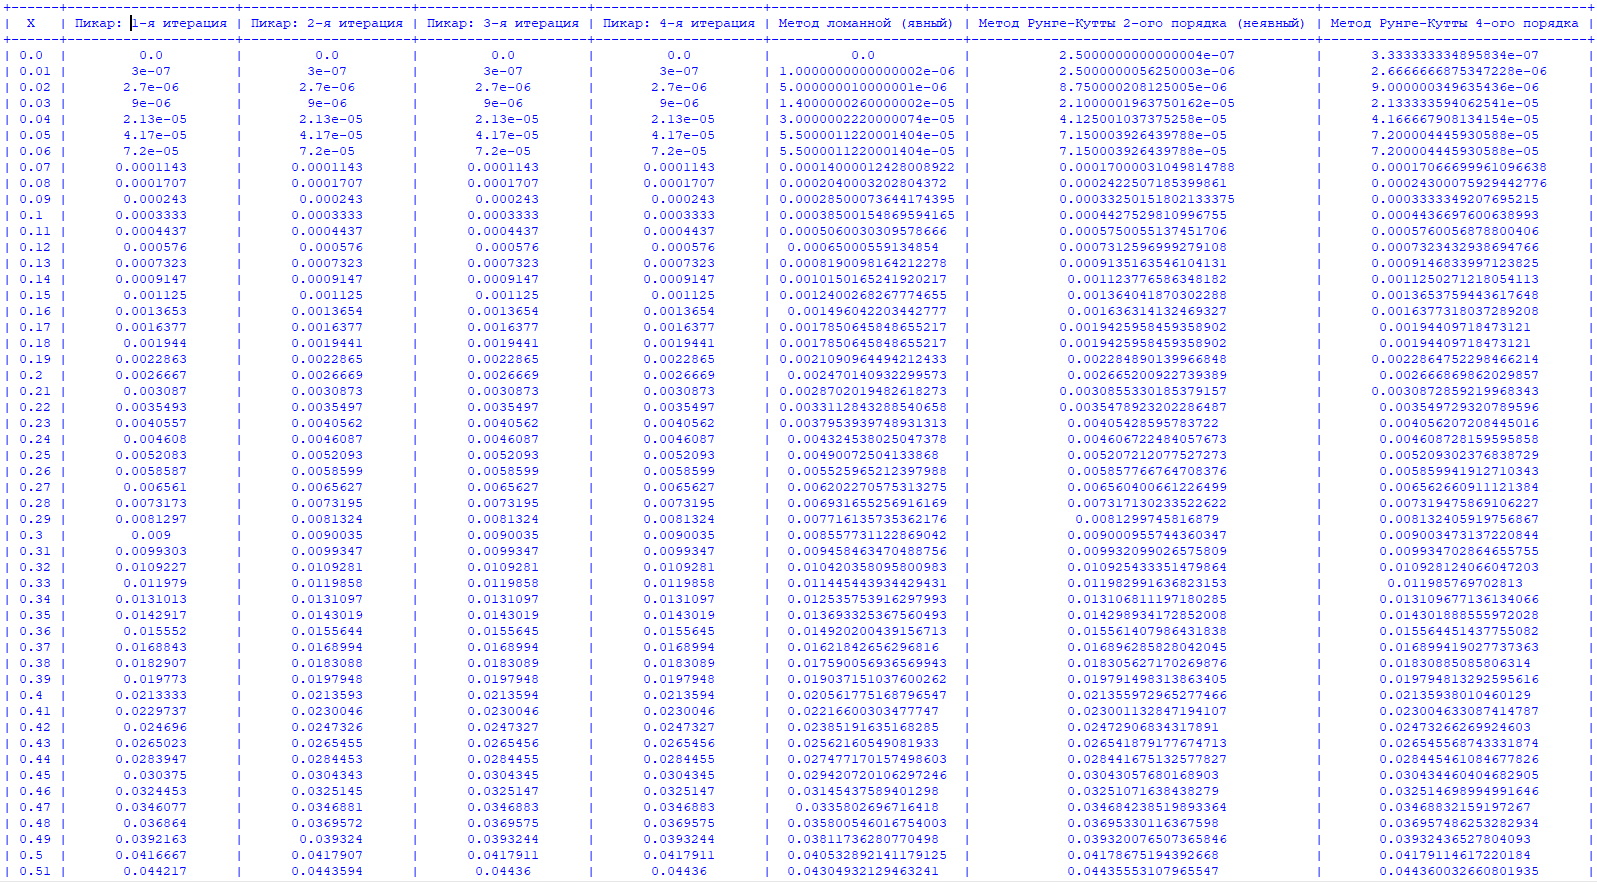
\includegraphics[width=7.0in]{../pics/1.png}	
	
	\section{Понятие математической модели. Функции моделей. Источники погрешностей при построении модели, алгоритмизации и программировании.}
	
	Математическая модель - это представление объекта на языке математики в виде уравнений, математических соотношений\\\\	
	Функции модели:
	\begin{enumerate}
		\item Познание. Прежде чем разрабатывать модель, нужно получить информационное оснащение (матер. коэффициенты) - расчетами или из экспериментов. Чем более детально описываем процесс, тем больше нужно доп информации. 
		\item Прогнозирование (предсказание). Например, можем узнать, что произойдет, если начнется, ядерная война или упадет астероид. Прогнозирование -> оптимизация.
		\item Модель - это компактный и удобный способ передачи информации. При моделировании систем - передача информации между подсистемами. 
		\item Тренажеры. 
	\end{enumerate}

	\section{Понятие корректности постановки задач. Привести примеры некорректно поставленных и слабо обусловленных задач и  неустойчивых алгоритмов. }
	Задача называетсякорректно поставленной, если решение существует, еднственно и непрерывно зависит от начальных данных. 
	\begin{equation}
	 y = Ax 
	 \end{equation}
	\begin{equation}
 		\sigma x -> \sigma y -> 0
	\end{equation}
	Если задача некорректна, малое изменение $\sigma x$ приведет к большому $\sigma y$. То есть малое изменение погрешности входных данных приведет к большому изменению погрешности результата.\\\\	
	Пример некорректной задачи:
	$\sigma y = C \sigma x $, где $C >> 0$ (слабоустойчивая задача).\\
	Для решение - Регуляризация.\\\\	
	Виды погрешностей моделирования:\\
	1) погрешность исходных данных\\
	2) погрешность метода и алгоритма\\
	3) погрешость окружения\\
	4) погрешность самой модели\\\\	
	Помимо неустойчивости формулировки задачи, может быть неустойчив сам алгоритм.\\\\
	Пример:\\
	$u'(x) = - \alpha u, \alpha > 0 $\\
	$u (x) = u_0\exp^{\alpha x}$\\\\
	По оХ выберем сетку с постоянным шагом h. \\\\
	$u (x) -> y,  u (x_i) -> y_i$\\
	$y_{n+1} = y_n + hu'_n = y_n + h(-\alpha y) = y_n (1 - h\alpha) $\\\\
	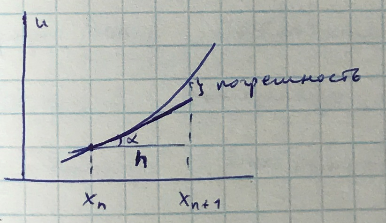
\includegraphics{../pics/2.png}\\
	\\Если  $(1 - h\alpha) < 0 $ ,  то $y_n$ меняет знак.\\
	\\ 
	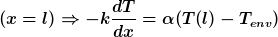
\includegraphics{../pics/3.png}\\
	\\Пилообразное решение. Чтобы такого не было, накладываем ограничение на h:\\
	$h < \frac{1}{\alpha}$\\
	Получаем относительно устойчивое решение.
	\\
	$y_{n+1} = y_n + h u'_{n+1} = y_n + h (-\alpha y_{n+1})$\\
	$y_{n+1} (1 + \alpha h) = y_n$\\
	$y_{n+1} = \displaystyle \frac{y_n}{1 + \alpha h}$ - грубое решение, но пилообразных разных результатов не получим.\\
	
	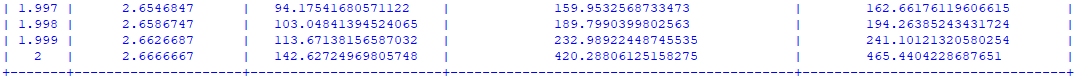
\includegraphics{../pics/4.png}
	
	\section{Общая классификация методов построения математических моделей.}
	Методы получения математических моделей:
	\begin{enumerate}
		\item На основе фундаментальных законов природы 
		\item Из вариационных принципов (принцип Гамельтона, Ферма (оптика))		
		\item Выстраивание иерархии моделей (построить простую, потом усложнить)
		\item Метод аналогии		
	\end{enumerate}
	Пример:\\
	Модель, которая показывает как 

	\section{Построение математических моделей на основе законов природы. Привести примеры.}
	Наиболее распространенный метод построения моделей состоит в применении фундаментальных законов природы к конкретной ситуации (ЗСЭ, ЗСИ). Вопрос в том, , какой закон (законы) следует применять в данном случае и как это делать. \\
	Пример: траектория всплытия подводной лодки.\\
	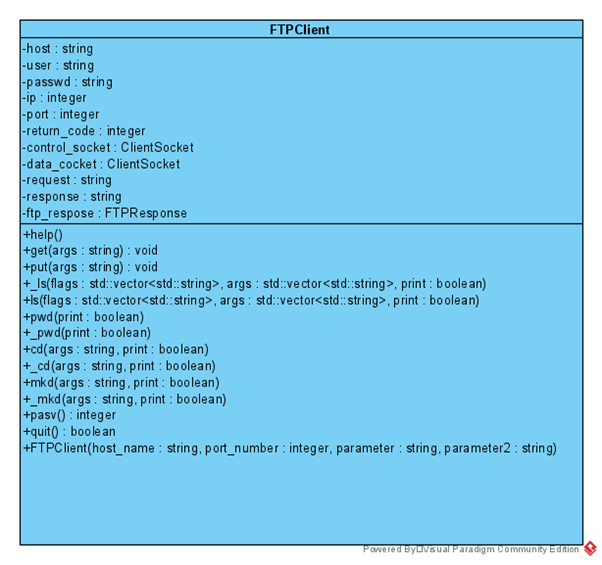
\includegraphics{../pics/5.png}\\
	Пусть подводная лодка, находящаяся в момент времени  t = 0 на глубине Н от поверхности моря и движущаяся с постоянной горизонтальной скоростью v, получает приказ подняться на поверхность. Если промежуток времени, за который уистерны подлодки освобождаются от воды и заполняются воздухом, с тем чтобы ее средняя плотность $\rho_1$  стала меньше плотности воды $\rho_0$, невелик, то можно можно считать, что в t = 0 на подлодку начинает действовать выталкивающая сила, большая, чем вес лодки. \\
	По закону Архимеда $ F = g V \rho_0$. \\
	Суммарная сила, действующая на подлодку в вертикальном направлении, - разность между F и весом тела $P = g V \rho_1$, а сообщаемое ею ускорение по второму закону Ньютона равно \\
	$\rho_1  V \displaystyle\frac{d^2 h}{d t^2}= F - P = g V (\rho_0 - \rho_1)$\\
	Координата l, характеризующая горизонтальное положение подлодки, изменяется по закону движения тела с постоянной скоростью: \\
	$\displaystyle\frac{d l}{d t} = v$\\
	Решая уравнения, находим, что:\\
	$h(t) = g\displaystyle\frac{(\rho_0-\rho_1)}{\rho_1} t^2 , l(t) = v t$  (1)\\
	И что лодка всплывет на поверхность в $t = t_k$, когда\\
	$h(t_k) = g\displaystyle\frac{(\rho_0-\rho_1)}{\rho_1} t^2_k , t_k = (\frac{\rho_1 H}{g(\rho_0-\rho_1)})^{1/2}$\\
	При этом в горизонтальном направлении подлодка пройдет расстояние\\
	$L = v t_k = (\displaystyle\frac{\rho_1 H}{g(\rho_0-\rho_1)})^{1/2}$\\
	Исключая из (1) время, найдем траекторию движения подлодки в координатах (l, h)\\
	$h = g\displaystyle\frac{\rho_0-\rho_1}{\rho_1 v^2} l^2$	\\
	которая оказывается параболой с вершиной в точке l = 0, h = 0 \\
	Итак, применение закона Архимеда и закона Ньютона позволило найти траекторю подлодки. Параболической траекторией обладает любое движующееся в плоскости тело, имещее по одному из направлени постоянную скорость и на которое в другом направлении действует постоянная сила (полет камня, брошенного с высоты Н с горизонтальной скоростью v или полет электрона в эл поле плоского конденсатора). 
	
	
	\section{Построение математических моделей на основе вариационных принципов. Привести примеры.}
	Движение шарик, присоединенного к пружине.\\
	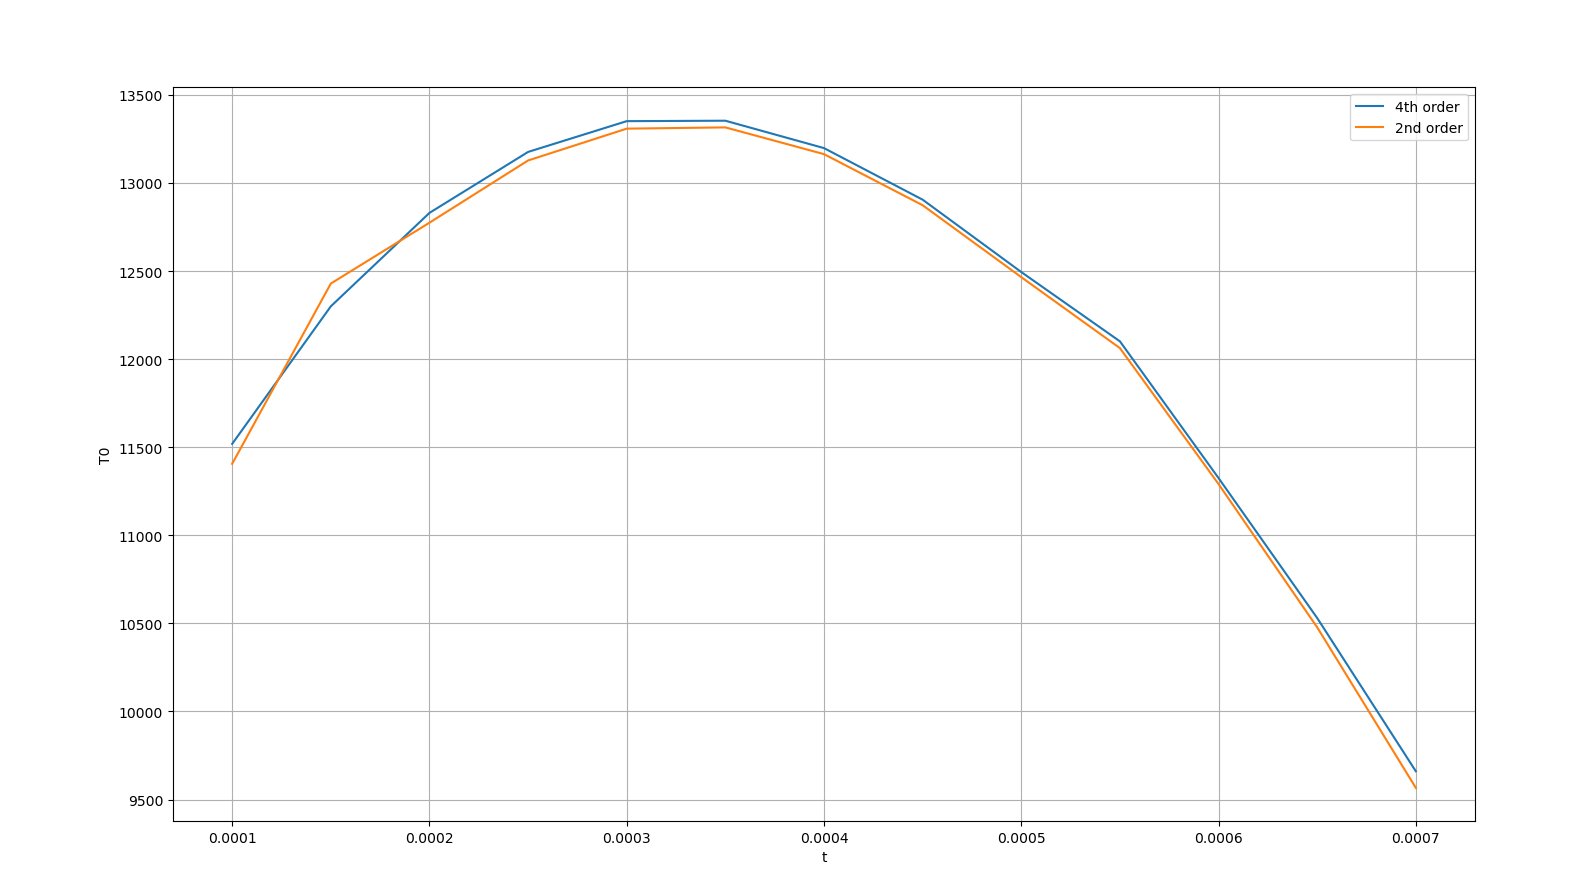
\includegraphics{../pics/6.png}\\
	Пусть $r$ - координата шарика вдоль оси пружины, лежащей на горионтальной плоскости, и направление движения шарика совпадает с ее осью. Тогда по второму заокнму динамики:\\
	$F = m a = m \displaystyle\frac{d^2r}{dt^2}$\\
	Единственная сила, действующая на шарик в направлении оси r - сила упругости пружины. Определим ее, используя закон Гука:\\
	$F = -kr$\\
	Уравнение движения шарика принимает вид (уравнение элементарного осциллятора):\\
	$m\displaystyle\frac{d^2r}{dt^2} = -kr$\\
	Оно описывает его гармонические колебания и имеет общее решение \\
	$r = A \sin \omega t + B \cos \omega t$,\\
	где $\omega = \sqrt{\displaystyle\frac{k}{m}} $ - частота колебаний . \\
	Воспользуемся принципом Гамильтона (общая схема) для построения модели движения шарика. В качестве обобщенной координаты выберем эйлерову координату шарика $r(t)$. Тогда обобщенная скорость $\frac{dr}{dt} = v(t)$ - обычная скорость шарика.Фнукция Лагранжа $ L = E_k - E_n $ записывается через значения кинетической и потенциальной энергии системы. \\
	$L = \displaystyle\frac{m(\displaystyle\frac{dr}{dt})^2}{2} - k\displaystyle\frac{r^2}{2}$\\
	Для величины действия получаем выражение:\\
	$S[r] = \displaystyle\int_{t_1}^{t_2} L(r, dr/dt) dt = \displaystyle\int_{t_1}^{t_2}[\displaystyle\frac{m}{2}(\displaystyle\frac{dr}{dt})^2 - \displaystyle\frac{k}{2}r^2] dt $\\
	Теперь вычислим действие на вариациях $\varepsilon\varphi(t)$ координаты r(t):\\
	\begin{equation*}
	S[r+\varepsilon\varphi] = \int_{t_1}^{t_2}\left[\frac{m}{2}(\frac{d(r+\varepsilon\varphi)}{dt}) - \frac{k}{2}(r+\varepsilon\varphi)^2\right]dt
	\end{equation*}
	Последнюю формулу необходимо продифференцировать по $\varepsilon$ (учитывая, что функции $r, \varphi, dr/dt, d\varphi/dt$ от $\varepsilon$ не зависят):\\
	\begin{eqnarray}
	\frac{d}{d\varepsilon}S[r+\varepsilon\varphi] = \frac{d}{d\varepsilon} \frac{1}{2}  \int_{t_1}^{t_2}\left[m\left\{(\frac{dr}{dt})^2 + 2\varepsilon\frac{dr}{dt}\frac{d\varphi}{dt} + \varepsilon^2(\frac{d\varphi}{dt})^2\right\} - k\{r^2 + 2\varepsilon r\varphi + \varepsilon^2\varphi^2\}\right]dt = \nonumber \\
	 = \int_{t_1}^{t_2}\left[m\left\{\frac{dr}{dt}\frac{d\varphi}{dt} + \varepsilon(\frac{d\varphi}{dt} )^2 \right\} - k\{r\varphi+\varepsilon\varphi^2\} \right] dt
	\end{eqnarray}
	и положить в ней $\varepsilon = 0$ :\\
	\begin{equation*}
	\frac{d}{d\varepsilon}S[r+\varepsilon\varphi]\Bigl|_{\varepsilon=0} = \int_{t_1}^{t_2}\left[m\frac{dr}{dt}\frac{d\varphi}{dt} -kr\varphi\right] dt = 0
	\end{equation*}
	Правая часть этого выражения (равного нлю в согласии с принципом Гамильтона) с помощью интегрирования ее первого члена по частям и с учетом того, что $\varphi=0$ в моменты $t_1, t_2$, преобразуется к виду \\
	\begin{equation*}
	\frac{d}{d\varepsilon}S[r+\varepsilon\varphi]\Bigl|_{\varepsilon=0} = -\int_{t_1}^{t_2}\varphi\left[m\frac{d^2r}{dt^2} +kr\right] dt = 0
	\end{equation*}
	Поскольку пробная функция $\varphi(t)$, фиурирующая в формулировке принципа наименьшего действия, произвольна, то часть выражения, стоящая под знаком интеграла в квадратных скобках, должна быть равна нулю  во все моменты времени $t_1 < t < t_2$:\\
	\begin{equation*}
	m\frac{d^2r}{dt^2} = -kr
	\end{equation*}
	\section{Построение математических моделей выстраиванием иерархии сверху - вниз и снизу - вверх. Привести примеры.}
	Естествен подход, реализующий принцип "от простого — к сложному", когда следующий шаг делается после достаточно подробного изучения не очень сложной модели. При этом возникает цепочка ( иерархия ) все более полных моделей, каждая из которых обобщает предыдущие, включая их в качестве частного случая.\\\\	
	Построим такую иерархическую цепочку на примере модели многоступенчатой ракеты. Реальная одноступенчатая ракета неспособна развить первую космическую скорость. Причина этого - затраты горючего на разгон ненужной, отработавшей части структурной массы. Следовательно, при движении ракеты необходимо периодически избавляться от балласта. В практической конструкции это означает, что ракета состоит из нескольких ступеней, отбрасываемых по мере их использования.\\
	Пусть $m_i$ - общая масса i-й ступени, $\lambda m_i$ - соответствующая структурная масса ( при этом масса топлива равна величине $(1 - \lambda)m_i$, $m_p$ - масса полезной нагрузки. Величины $\lambda$ и скорость истечения газов одинаковы для всех ступеней. Возмем для определенности число ступеней n = 3. Начальная масса такой ракеты равна  \\
	$m_0 = m_p + m_1 + m_2 + m_3$\\
	Рассмотрим момент, когда израсходовано все топливо первой ступени и масса ракеты равна величине\\
	$m_p + \lambda m_1 + m_2 + m_3$\\
	Тогда по формуле первоначальной модели\\
	$v = u ln(\displaystyle\frac{m_0}{m_p + m_s}) $, $m_s$ - структурная масса\\
	скорость ракеты равна\\
	\begin{equation*}
	v_1 = u ln\left(\frac{m_0}{m_p + \lambda m_1 + m_2 + m_3}\right)
	\end{equation*}	
	После достижения скорости $v_1$ структурная масса $\lambda m_1 $ отбрасывается и включается вторая ступень. Масса ракеты в этот момент равна \\
	$m_p + m_2 + m_3$\\
	Начиная с этого момента и до момента полного выгорания топлива второй ступени , ничто не мешает пользоваться уже построенной моделью, применив ее к рассматриваемому случаю. Все рассуждения о сохранении суммарнго импульса и соответствующе выкладки отстаются в силе ( следует только учесть, что у ракеты уже есть начальная скорость  $v_i$). Тогда после выгорания топлива во второй ступени ракеты достигает скорости\\
	\begin{equation*}
	v_2 = v_1 + u ln\left( \frac{m_p + m_2 + m_3}{m_p + \lambda m_2 + m_3}\right)
	\end{equation*}
	Такие же рассуждения применинмы и к третьей ступени ракеты. После отключения ее двигателей скорость ракеты равна \\
	\begin{equation*}
	v_3 = v_2 + u ln\left(\frac{m_p + m_3}{m_p + \lambda m_3} \right)
	\end{equation*}
	В случае трех ступеней для окончательной скорости имеем\\
	\begin{equation*}
	\frac{v_3}{u} = ln\left(\frac{m_0}{m_p + \lambda m_1 + m_2 + m_3}\right)\left( \frac{m_p + m_2 + m_3}{m_p + \lambda m_2 + m_3}\right)\left(\frac{m_p + m_3}{m_p + \lambda m_3}\right)
	\end{equation*}
	или вводя величины $\alpha_1, \alpha_2, \alpha_3$ для выражений внутри логарифма, получаем:\\
	\begin{equation*}
	\frac{v_3}{u} = ln\left\{ \left(\frac{\alpha_1}{1+\lambda(\alpha_1-1)}\right)\left(\frac{\alpha_2}{1+\lambda(\alpha_2-1)}\right)\left(\frac{\alpha_3}{1+\lambda(\alpha_3-1)}\right)\right\}
	\end{equation*}
	Данное выражение симмтерично по отношению к величинам $\alpha_1, \alpha_2, \alpha_3$ и нетрудно показать, что его максимум достигается в симметричном случае, т.е. при $\alpha_1 = \alpha_2 \ \alpha_3$. При этом для i = 3\\
	$\alpha = \displaystyle\frac{1-\lambda}{P - \lambda}$ , $P = \exp\left(-\displaystyle\frac{v_3}{3u}\right)$\\
	Произведение $\alpha_1\alpha_2\alpha_3 = \alpha$ равно отношению $\frac{m_0}{m_p}$ или \\
	$\alpha^3 = \displaystyle\frac{m_0}{m_p} = \left(\displaystyle\frac{1-\lambda}{P - \lambda}\right)^3$\\
	Для многоступенчатой ракеты имеем:\\
	$\displaystyle\frac{m_0}{m_p} = \left(\displaystyle\frac{1-\lambda}{P - \lambda}\right)^n$\\
	Таким образом иерархия математических моделей от простого к сложного позволила относительно легко прийти к этим выводам. 
	\section{Построение математических моделей методом аналогий. Привести примеры.}
	В огромном числе случаев при попытке построить модель какого-либо объекта либо невозможно прямо указать фундаментальные законы или вариационные принципы, которым он подчиняется, либо, с точки зрения наших сегодняшних знаний, вообще нет уверенности в существовании подобных законов, допускающих математическую формулировку. Одним из плодотворных подходов к такого рода объектам является использование аналогий с уже изученными явлениями.\\
	Пример:\\
	Модель, которая поазывает как изменитяс популяция людей.\\
	$n(t, x)$ - количество людей, Х - возраст\\
	$\displaystyle\frac{\partial n}{\partial t} + \displaystyle\frac{\partial n}{\partial x} = - \alpha(x) n$\\
	$\alpha$ - коэффициент смертности\\
	Краевое условие задаем x = 0:\\
	$n(t, 0) = \displaystyle\int_{x_1}^{x_2}\beta(x, t) n(x, t) dx$\\
	Это уравнения переноса интенсивности. Применим аналогию. 
	\section{Понятие ОДУ. Сведение ОДУ произвольного порядка к системе ОДУ первого порядка. Привести примеры.}
	ОДУ - уравнения, которые содержат одну независимую переменную. Если переменных несколько, то это уравнения в частных производных. \\
	\begin{equation*}
	u^{(n)}(x) = f(x, u, u' ,u'', ..., u^{(n-1)})
	\end{equation*}
	Заменой переменных . уравнение n-го порядка может быть сведено к системе n уравнений 1-го порядка. Как :\\\\
	$u^{(k)} = u_k$\\\\
	$u'_k = (u^{(k)})' = u^{(k+1)} = u_{k+1}$\\\\
	$\begin{cases}
	u'_k &= u_{k+1}, 0 <= k <= n-2, u(x) = u_0(x)\\
	u'_{n-1}(x) &= f(x, u_0, u_1, ..., u_{n-1}) 
	\end{cases}$\\\\

	\section{Постановка задачи Коши для системы ОДУ первого порядка.}
	В общем случае 	система ОДУ 1-го порядка выглядит так:\\
	$u'_k(x) = f_k(x, u_1, u_2, .., u_n)$ , $k = \overline{1, n}$ \\\\
	Задача Коши: \\из системы общих решений системы ОДУ выделяют единтвенное решение.\\ В задаче Коши  все дополнительные условия для выделения частного решения ставятся в одной точке.\\\\
	$u_k(\xi) = \eta_k$ , $k = \overline{1, n}$\\\\
	Методы решения:\\
	1) Аналитические\\\
	2) Приближенные аналитические\\
	3) Численные\\
	\section{Постановка краевой задачи для ОДУ.}
	Общий вид системы ОДУ первого порядка\\\\
	$u'_k(x) = f_k(x, u_1, u_2, .., u_n)$ , $k = \overline{1, n}$ \\\\
	$u' = u_1$	$u'' =  u_2$\\\\
	Задача нахождения функции u = u(x) из условий \\\\
	$u''  + a_1(x)u' + a_2(x)u = f(x)$\\\\
	Краевая задача - задача нахождения решения ОДУ, удовлетворяющего краевым условиям в концах интервала или на границе области.
	
	\section{Задача Коши для ОДУ . Метод Пикара при решении ОДУ.  Привести пример.}
	Приближенный аналитический метод - метод Пикара.\\\\
	\begin{eqnarray*}
	u'(x) = f(x, u) \nonumber \\
	u(x) = u(0) + \int_{0}^{x}f(t, u(t)) dt
	\end{eqnarray*}
	Итерационная схема Пикара - задаче наччальные условия, подставляемв правую часть и итерационн решаем.
	\begin{equation*}
	y^{(s)}(x) = u(0) + \int_{0}^{x} f(t, y^{(s-1)}(t)) dt,   y^{(0)}(t) = u(0)
	\end{equation*}
	Метод сходится, это можно доказать. \\
	Условие сходимости:\\\\
	Область ограничена: $a <= x <= b; c <= u <= d$\\\\
	Функция $f(t, u(t))$ по 2-ому аргументу удовлетворяет условию Липшица:\\
	\begin{eqnarray*}
	\Bigl|f(x-1, u_1)- f(x_2, u_2) \Bigl| <= L\Bigl|u_1 - u_2\Bigl| \nonumber \\
	z^{(s)}(x) = \Bigl| u(x) - y^{(1)}(x)\Bigl| - \text{погрешность при} s->\infty , t^{(s)}(x)-> 0
	\end{eqnarray*}
	\\Пример\\
	\bigskip\noindent
	\begin{align*}
	\begin{cases}	
		&u'(x0) = x^2 + u^2  \\
		&u(0) = 0  
	\end{cases}\\\\
		&y^{(1)}(x) = 0 + \int_{0}^{x} t^2 dt = \frac{x^3}{3}\\
		&y^{(2)}(x) = 0 + \int_{0}^{x} \left[t^2 + \left(\frac{t^3}{3}\right)^2\right] dt = \frac{x^3}{3} + \frac{x^7}{9 \cdot 7} \\
		&y^{(3)}(x) = 0 + \int_{0}^{x} \left[t^2 + \left(\frac{t^3}{3} + \frac{x^7}{9 \cdot 7}\right)^2\right] dt = \frac{1}{3}x^3 \left( 1 + \frac{1}{21}x^4 + \frac{2}{693}x^8 + \frac{1}{19845}x^{12}\right) \\
	\end{align*}
	\\явный метод $y_{n+1} = y_n + hf(x_n, y_n)$\\
	\\неявный метод $y_{n+1} = y_n + hf(x_{n+1}, y_{n+1})$
	\section{Задача Коши для ОДУ. Метод Рунге - Кутта 2-го порядка точности. Оценка точности.}
	\textbf{Метод Рунге - Кутта.}
	\begin{align*}
	u'(x) &= f(x, u)\\
	u(\xi) &= \eta
	\end{align*}
	Выберем сетку  с постоянным шагом по x
	\begin{align*}
	&\omega: {a = x_0 < x_1 < x_2 < ... < x_n < x_{n+1} < ... < x_N = b}\\
	&\omega_h = {x_n = a + nh,  	n = \overline{1, N}}
	\end{align*}
	Фиксируется $x = a + nh = x_n$ , $h -> 0 (n -> \infty)$. \\
	Сеточное решение сходитсся к точному в точке x, если $ |u(x_n) - y_n| -> 0 , h -> 0$\\
	Сеточное решение сходится к точному на отрезке $[a, b]$б если оно сходится в каждой точке этого отрезка.\\\\
	Разностное (сеточное) решение сходится к точному с порядком p, если \\
	$|u(x_n) - y_n| = O(h^p) $ при $h -> 0$\\\\
	Введем сетку : $x_{n-1}, x_n, x_{n+1}$
	\begin{align*}
	&u_{n+1} \equiv  u_{(x_{n+1})}\\
	&u_{n+1} = u_n + hu'_n + \frac{h^2}{2}u''_n + \frac{h^3}{3!}u'''_n + ...\\
	&u'_n = u'(x_n) = f(x_n, u_n)\\
	&u''_n = \frac{df(x, u)}{dx} \Bigl|{x=x_n} = f'_x(x_n, u_n) + f'_u u'_x = f'_x(x_n, u_n) + f'_u f(x_n, u_n)
	\end{align*}
	\textbf{Метод Рунге-Кутта 2-го порядка точности.}\\
	\begin{align}
	&y_{n+1} = y_n + hu'_n + \frac{h^2}{2}u''_n\\
	&y_{n+1} = y_n + h f(x_n, y_n) + \frac{h^2}{2} (f'_x + f'_nf) \Bigl|_{x_n, y_n}\\
	&u''_n = \frac{f(x_n + j h, y_n + \delta h) - f(x_n, y_n)}{\triangle  x}\\
	&y_{n+1} = y_n + h f(x_n, y_n) + \frac{h^2}{2 \triangle x} f (x_n + j h, y_n + \delta h) - \frac{h^2}{2 \triangle x} f(x_n, y_n) = y_n + h \beta f(x_n, y_n) + \alpha h f(x_n + j h, y_n + \delta h)\\
	&y_{n+1} = y_n + h \left[ \beta f(x_n, y_n) + \alpha f(x_n, + j h, y_n + \delta h)  \right] = y_n + h \left[ \beta f (x_n, y_n) + \alpha (f(x_n, y_n) + f'_x j h + f'_n \delta h) \right] \\
	&y_{n+1} = y_n + h \left[ (\alpha + \beta) f(x_n , y_n) + \alpha h (f'_x j + f'_n \delta)\right]
	\end{align}\\
	Чтобы (8) перешло в (5) надо, чтобы:\\
	\begin{equation*}
	\begin{cases}
		\alpha + \beta &= 1\\
		\alpha y &= \frac{1}{2}\\
		\alpha \delta &= \frac{1}{2} f(x_n, y_n)
	\end{cases}
	\end{equation*}\\
	$\alpha$ - свободный параметр. Остальное находим через него. \\
		\begin{equation*}
	\begin{cases}
		\beta &= 1 - \alpha\\
		j &= \frac{1}{2\alpha}\\
		\delta &= \frac{1}{2\alpha} f(x_n, y_n)\\
	\end{cases}	
	\end{equation*}\\
	\begin{align*}
	&y_{n+1} = y_n + h \left[ ( 1 - \alpha) f(x_n, y_n) + \alpha f(x_n + \frac{h}{2\alpha}, y_n + \frac{h}{2\alpha}f(x_n, y_n))\right]\\
	\end{align*}\\
	Порядок точности $O(h^2)$\\
	На практике $\alpha = 1$ или $\alpha = \frac{1}{2}$\\\\
	Геометрическая интерпретация при $\alpha = 1$\\
	\begin{align*}
	y_{n+1} = y_n + h f(x_n + \frac{h}{2}, y_n + \frac{h}{2} f(x_n, y_n))\\
	\end{align*}\\\\
	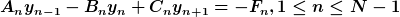
\includegraphics{../pics/7.png}\\
	\begin{align*}
	&1. y_{n+1/2} = y_n + \frac{h}{2}f(x_n, y_n)\\
	//&\triangle u = u(x_{n+1}) - y_{n+1} (\text{метод ломаных явный})\\
	&2. y'_{n+1/2} = f(x_{n+1/2}, y_{n+1/2})\\
	&3. y_{n+1} = y_n +  h y'_{n+1/2}\\
	&\text{При } \alpha = \frac{1}{2}:\\
	&y_{n+1} = y_n = \frac{h}{2} \left[f(x_n, y_n) + f(x_n + h, y_n + hf(x_n, y_n))\right]\\
	\overline{y_{n+1}} = y_n + h f(x_n, y_n)\\
	\end{align*}
	\section{Задача Коши для ОДУ. Метод Рунге - Кутта 4-го порядка точности. Оценка точности.}
	\textbf{Метод 4-го порядка: }\\
	\begin{align*}
	&y_{n+1} = y_n + \frac{h}{6} (k_1 + 2k_2 + 2k_3 + k_4)\\
	&k_1 = f(x_n, y_n)\\
	&k_2 = f(x_n + \frac{h}{2}, y_n + \frac{k_1h}{2})\\
	&k_3 = f(x_n + \frac{h}{2}, y_n = {hk_2}{2})\\
	&k_3 = f(x_n + h, y_n + hk_3)\\
	\end{align*}\\
	Погрешность $O(h^4)$\\
	\begin{align*}
	&u'(x) = f(x)\\
	&y_{n+1} = y_n + \int_{x_n}^{x_{n+1}}f(x) dx\\	
	\end{align*}
	\textbf{Метод Рунге Кутта 4-го порядка: }\\
	//Формула Симпсона\\
	\begin{align*}
	&y_{n+1} = y_n + \frac{h}{6} \left[ f(x_n) + 4f(x_N  + \frac{h}{2}) + f(x_n + h)\right]\\	
	\end{align*}\\
	Погрешность формулы Симпсона $R_n \approx - \displaystyle\frac{h^4}{2600}\int_{x_n}^{x_{n+1}}f^{iv}(t)dt$\\\\
	Обобщение метода РК на случай 2-х переменных\\
	\begin{align*}
	\begin{cases}
	u'(x) = f(x, u, v), &u(x_n) = y_n\\
	v'(x) = \varphi(x, u, v), &v(x_n) = v_n\\
	u(\xi) = \eta_1, &y_{n+1} = y_n + \frac{h}{6}(k_1 + 2k_2 + 2k_3 + k_4)\\
	u(\xi) = \eta_2, &z_{n+1} = z_n + \frac{h}{6}(p_1 + 2p_2 + 2p_3 + p_4)
	\end{cases}
	\end{align*}
	где 
	\begin{align*}
	k1 &= f(x_n, y_n, z_n)\\
	p1 &= \varphi(x_n, y_n, z_n)\\
	k2 &= f(x_n + \frac{h}{2}, y_n + \frac{h}{2}k1, z_n + \frac{h}{2}p1)\\
	p2 &= \varphi(x_n + \frac{h}{2}, y_n + \frac{h}{2}k1, z_n + \frac{h}{2}p1)\\
	k3 &= f(x_n + \frac{h}{2}, y_n + \frac{h}{2}k2, z_n + \frac{h}{2}p2)\\
	p3 &= \varphi(x_n + \frac{h}{2}, y_n + \frac{h}{2}k2, z_n + \frac{h}{2}p2)\\
	k4 &= f(x_n + h, y_n + hk3, z_n + hp3)\\
	p4 &= \varphi(x_n + h, y_n + hk3, z_n + hp3)\\
	\end{align*}
	\section{Задача Коши для ОДУ. Метод Адамса.}
	Для решения ОДУ или систем ОДУ существуют одностадийные методы Адамса (линейные многошаговые методы) (многошаговые в отличие от одношаговых учитывают несколько предыдущих значений), суть которых заключается в следующем.\\	
	Пусть известно приближенное решение в некоторых узлах расчетной сетки: tn, tn - 1, ..., tn - m. В окрестности этих узлов заменим f(t, x(t)) интерполяционным полиномом\\
	\begin{align*}
	f(t) = f(t_n) + &f(t_n, t_{n-1})(t-t_n)+\\
	&f(t_n, t_{n-1},t_{n-2})(t-t_{n-1})+\\
	&f(t_n, t_{n-1},t_{n-2}, t_{n-3})(t-t_n)(t-t_{n-1})(t-t_{n-2})+... \\
	\end{align*}
	Для того чтобы вычислить решение в точке $n + 1$, запишем его в интегральном виде\\
	\begin{equation*}
	u_{n+1} = u_n + \int_{t_n}^{t_{n+1}} f(t,u(t))dt = \int_{t_n}^{t_{n+1}}f(t)dt
	\end{equation*}\\
	и подставим в него интерполяционный полином с переменным шагом\\
	\begin{align*}
	u_{n+1} = u_n + \tau_n f(t_n) + &\frac{\tau^2_n}{2}f(u_n, u_{n-1}) + \\
	 &\frac{\tau^2_n}{6}(2\tau_n + 3\tau_{n-1})f(u_n, u_{n-1}, u_{n-2}) + \\
	 &\frac{\tau^2_n}{12}(2\tau^2_n+8\tau_n\tau_{n-1}+4\tau_n\tau_{n-2} + 6\tau^2_{n-1} + 6\tau_n\tau_{n-2})f(u_n, u_{n-1}, u_{n-2}, u_{n-3})
	\end{align*}\\
	здесь\\
	\begin{equation*}
	\tau_n = t_{n+1} - t_n, f(u_n, u_{n-1}), f(u_n, u_{n-1}, u_{n-2})
	\end{equation*}
	разделенные разности\\
	Эта формула четвертого порядка точности. Если опустить последнее слагаемое, то получим формулу третьего порядка, если опустить еще и предпоследнее, то — второго, и т.д.\\
	Для того чтобы начать вычисления по данному варианту метода Адамса, необходимо знать решение в четырех точках. Это можно сделать, например, с помощью методов Рунге - Кутты. Кроме того, коэффициент при погрешности, например, для метода четвертого порядка точности Рунге - Кутты существенно меньше соответствующего коэффициента для метода Адамса.\\\\	
	Первые четыре метода Адамса, от первого до четвертого порядка точности с постоянным шагом интегрирования, представляются в виде\\
	\begin{align*}
	&u_{n+1} = u_n + \tau f_n\\
	&u_{n+1} = u_n + \tau (\frac{3}{2}f_n - \frac{1}{2}f_{n-1})\\
	&u_{n+1} = u_n + \tau (\frac{23}{12}f_n - \frac{16}{12}f_{n-1} + \frac{5}{12}f_{n-2})\\
	&u_{n+1} = u_n + \tau (\frac{55}{24}f_n - \frac{59}{24}f_{n-1} + \frac{37}{24}f_{n-2} - \frac{9}{24}f_{n-3})\\
	\end{align*}
	В общем виде методы Адамcа могут быть записаны следующим образом:\\
	\begin{align*}
	u_{n+1} = u_n + \tau \sum_{j=0}^{k-1}\eta_j \triangle^j f_j
	\end{align*}
	\section{Задача Коши для ОДУ. Неявные численные методы (Эйлера, трапеций,  Гира). }
	Неявные методы:\\
	\begin{enumerate}
		\item Метод Эйлера 
		\begin{align*}
		y_{n+1} = y_n + f(x_{n+1}, y_{n+1}) , \text{Сложность } O(h)\\
		\end{align*}
		\item Метод трапеций\\
		Проинтегрируем (1) методом трапеций
		\begin{align*}
		y_{n+1} = y_n + \frac{h}{2}\left[ f(x_n, y_n) + f(x_{n+1}, y_{n+1})\right] , \text{Сложность } O(h^2)\\
		\end{align*}
		Методы устойчивы. Проблема в том, как решать уравнение. Как найти решение $y^{(s)}_{n+1}$ - ?\\
		\begin{align*}
		&y^{(s)}_{n+1} = y_n + \frac{h}{2}\left[f(x_n, y_n) + f(x_{n+1}, y^{(s-1)}_{n+1})\right] \text{используем эту формулу.}\\
		&\varphi(x) = 0\\
		&x = \psi(x)\\
		&x^{(\varphi)} = \psi(x^{(\psi-1)}), |\psi'(\xi)| < 1 ! - \text{Условие сходимости}\\
		\end{align*} 
		\item Методы Гира\\
		\begin{align*}
		&\frac{3}{2}y_n - 2y_{n-1} + \frac{1}{2}y_{n-2} = hf(x_n, y_n) , O(h^2), y_n - \text{неизв}		\\		
		&\frac{11}{6}y_n - 3y_{n-1} + \frac{3}{2}y_{n-2} - \frac{1}{3}y_{n-3} = hf(x_n, y_n), O(h^3)
		\end{align*}
		Устойчивые методы
	\end{enumerate}
	\section{Краевая задача для ОДУ. Метод коллокаций. Привести пример.}
	\begin{align*}
	&u''(x) + p(x) u'(x) + g(x)u(x) = f(x)\\
	&Lu(x) = f(x)\\	
	\end{align*}
	L - оператор $(u''(x) + p(x)u'(x) + g(x)u(x)$\\
	p(x), g(x), f(x) - заданные функции\\
	Получаем аналитическое выражение. Краевые (граничные) условия:\\
	\begin{align*}	
	&a <= x <= b\\
	&\begin{cases}
	\varGamma_a u &= \alpha_0 u(a) + \beta_0 u'(a) = A\\
	\varGamma_b u &= \alpha_1 u(b) + \beta_1 u'(b) = B\\
	\end{cases}
	\end{align*}
	$u_0(x), u_1(x), ..., u_n(x)$ - базисные функции (они линейно независимы)\\
	$y(x) = u_0(x) + \sum_{k=1}^{n}C_k U_k(x)$\\
	$u_0(x)$ надо подобрать. Строится таким образом, чтобы она удовлетворяла краевым условиям.\\
	Все фукнции $u_k$ подбираются так, чтобы они удовлетворяли однородным краевым условиям (A = 0, B = 0).\\
	Подставим y в начальное уравнение \\
	\begin{align*}
	R(x, c_1, c_2, ..., c_n) = Ly - f = Lu_0(x) + \sum_{k=1}^{n}c_k L u_k(x) - f(x)
	\end{align*}
	Выбирают некоторое количество точек $c_1, ..., c_n$ в которых полагается невязка = 0:\\
	$R(x, c_1, ..., c_n) = 0$\\
	Пример:\\
	\begin{align*}
	&u'' + (1+x^2)u + 1 = 0\\
	&u(-1) = 0\\
	&u(+1) = 0\\
	\end{align*}
	Выбираем
	\begin{align*}
	&u_k(x) = x^{2k-2} (1 - x^2), k=\overline{1, n}\\
	&u_1(x), u_2(x)\\
	&y = c_1(1-x^2) + c_2(x^2 - x^4)\\
	&y'= -c_1 2x + 2c_2 (x - 2x^3)\\
	&y'' = -2c_1 + 2c_2 (1 - 6x^2)\\
	&R(x, c_1, c_2)  = -2_c1 + 2c_2 ( 1 - 6x^2) + (1+x^2) \left[ c_1(1-x^2) + c_2(x^2 - x^4) \right] + 1 = \\
	&= 1 - c_1(1+x^4) + c_2(2-11x^2-x^6)\\
	\end{align*}
	Выберем точки коллокаций\\
	$x = 0, x = 1/2$\\\\
	$1-\displaystyle\frac{17}{16}c_1 -\displaystyle\frac{49}{64}c_2 = 0$\\\\
	$c_1 = 0, 957, c_2 = -0,022$\\\\
	Итак, $y(x) \approx 0,957 (1-x^2) - 0,022 (x^2-x^4)$.\\
	Чем больше констант, тем точнее (но не всегда).
	\section{Краевая задача для ОДУ. Интегральный метод наименьших квадратов. Привести пример.}
	Постановка задачи:\\
	\begin{align*}
	&u''(x) + p(x) u'(x) + g(x)u(x) = f(x)\\
	&Lu(x) = f(x)\\	
	\end{align*}
	L - оператор $(u''(x) + p(x)u'(x) + g(x)u(x)$\\
	p(x), g(x), f(x) - заданные функции\\
	Получаем аналитическое выражение. Краевые (граничные) условия:\\
	\begin{align*}	
	&a <= x <= b\\
	&\begin{cases}
	\varGamma_a u &= \alpha_0 u(a) + \beta_0 u'(a) = A\\
	\varGamma_b u &= \alpha_1 u(b) + \beta_1 u'(b) = B\\
	\end{cases}
	\end{align*}
	Выбираем базис, который удовлетворяет граничнымусловим как в методе Коллокаций:\\
	$u_0(x), u_1(x), ..., u_n(x)$ - базисные функции (они линейно независимы)\\
	$y(x) = u_0(x) + \sum_{k=1}^{n}C_k U_k(x)$\\
	т.е. $u_0$ - неоднор. ГУ, $u_2, .., u_n$ - однородные\\
	Строим невязку , т.е. подставляем y в исходное уравнение\\
	\begin{align*}
	R(x, c_1, c_2, ..., c_n) = Ly - f = Lu_0(x) + \sum_{k=1}^{n}c_k L u_k(x) - f(x)\\
	\end{align*}
	Нужно, чтобы невязка была как можно меньше\\
	\begin{align*}
	\int_{a}^{b} R^2 dx -> min, \text{ т.е. } \int_{a}^{b} R\displaystyle\frac{\partial R}{\partial C_k}dx = 0, k=\overline{1, n}
	\end{align*}
	Пример \\
	\begin{align*}
	&u'' + (1+x^2)u + 1 = 0\\
	&u_1 = 1 - x^2, u_2  x^2 -x^4\\
	&y = c_1 ( 1-x^2)+ c_2(x^2-x^4)
	\end{align*}
	Находим R\\
	\begin{align*}
	&R(x, c_1, c_2) = 1 - c_1(1+x^4)+c_2(2-11x^2-x^6)\\
	&\frac{\partial}{\partial c_1}\int R^2 dx = \int_{0}^{1} \left[1 - c_1(1+x^4) + c^2(2 - 11x^2 -x^6)\right] \left[-(1+x^4)\right] dx = 0\\
	&\frac{\partial}{\partial c_1}\int R^2 dx = \int_{0}^{1} \left[1 - c_1(1+x^4) + c^2(2 - 11x^2 -x^6)\right] \left[2-11x^2-x^6\right] dx = 0\\
	&\frac{68}{45}c_1 + \frac{3548}{1155}c_2 = \frac{5}{4}\\
	&\frac{3548}{1155}c_1 + \frac{63404}{4055}c_2 = \frac{38}{21}\\
	&c_1 = 0,985\\
	&c_2 = -0,078
	\end{align*}
	Ответ\\
	\begin{align*}
	y(x) = 0,985(1-x^2) - 0,078(x^2-x^4)
	\end{align*}
	\section{Краевая задача для ОДУ. Дискретный метод наименьших квадратов. Привести пример.}
	В интегральном МНК имеем 
	\begin{align*}
	\int_{a}^{b} R^2 dx \rightarrow min
	\end{align*}
	Для рассмотренного примера 
	\begin{align*}
	\int_{0}^{1} \left[1 - c_1(1+x^4) + c^2(2 - 11x^2 -x^6)\right]^2 dx \rightarrow min
	\end{align*}
	Интеграл заменяем суммой\\
	Выбираем N точек на отрезке [0, 1] (на котором заданы краевые условия) : $x_i, i=\overline{1, N}$\\
	\begin{align*}
	&\phi(\overline{c}) = \sum_{i=1}^{N}R^2(x_i, \overline{c}) \rightarrow min\\
	&\frac{\partial\phi}{\partial c_1} = 0\\
	&\frac{\partial\phi}{\partial c_2} = 0\\
	&\frac{\partial\phi}{\partial c_3} = 0\\
	\end{align*}
	Если N - количество констант, то метод превращается в метод коллокаций. Поэтому берем $N >> n$ (хотя бы N = n+1). Для примера из интегрального МНК:\\
	\begin{align*}
	y(x) = 0,9317(1-x^2) - 0,0474(x^2-x^4)
	\end{align*}
	
	\section{Краевая задача для ОДУ. Метод Галеркина. Привести пример.}
	Постановка задачи:\\
	\begin{align*}
	&u''(x) + p(x) u'(x) + g(x)u(x) = f(x)\\
	&Lu(x) = f(x)\\	
	\end{align*}
	L - оператор $(u''(x) + p(x)u'(x) + g(x)u(x)$\\
	p(x), g(x), f(x) - заданные функции\\
	Получаем аналитическое выражение. Краевые (граничные) условия:\\
	\begin{align*}	
	&a <= x <= b\\
	&\begin{cases}
	\varGamma_a u &= \alpha_0 u(a) + \beta_0 u'(a) = A\\
	\varGamma_b u &= \alpha_1 u(b) + \beta_1 u'(b) = B\\
	\end{cases}
	\end{align*}
	Выбираем базис, который удовлетворяет граничнымусловим как в методе Коллокаций:\\
	$u_0(x), u_1(x), ..., u_n(x)$ - базисные функции (они линейно независимы)\\
	$y(x) = u_0(x) + \sum_{k=1}^{n}C_k U_k(x)$\\
	Находим невязку. Используем свойство:\\
	если $\displaystyle\int_{a}^{b}f(x) u_k(x) = 0, k = \overline{0, \infty}$, то $f(x) = 0$.\\
	\begin{align*}
	&\int_{a}^{b} R(x, c_1, c_2, ..., c_n) u_k(x) dx = 0, k=\overline{1,n}\\
	&\sum_{k=1}^{n} c_k \int_{a}^{b}u_k(x) L u_k(x) dx = \int_{a}^{b} u_k(x) \left[ f(x) - L u_0(x) \right] dx  \\\\
	&\begin{cases}
	u'' + xu' + u = 2x\\
	u(0) = 1 , u(1) = 0\\
	\end{cases}\\
	&u_0(x) = 1-x\\
	&u_1(x) = x (1-x)\\
	&u_2(x) = x^2(1-x)\\
	&u_3(x) = x^3(1-x)\\
	&y(x) = (1-x) + c_1 x(1-x) + c_2 x^2 (1-x) + c_3 x^3 (1-x)
	\end{align*}
	Невязка\\
	\begin{align*}
	R(x, c_1, c_2, c_3) = (1-4x) + c_1 (-2 + 2x - 3 x^2) + c_2 ( 2 - 6x + 3 x^2 - 4 x^3) + c_3 (6x - 12x^2 + 4x^3 - 5x^4)
	\end{align*}
	Далее\\
	\begin{align*}
	&\int_{0}{x} (x - x^2) R (x, \overline{c}) dx = 0, \overline{c} = \{c_1, c_2, c_3\}\\
	&\int_{0}{1} (x^2-x^3) R(x, \overline{c}) dx = 0\\
	&\int_{0}{1} (x^3-x^4) R(x, \overline{c}) dx = 0\\
	\end{align*}
	Вычисляя вышеописанные интегралы, подставляя невязку, получим систему уравнений:\\
	\begin{align*}
	\begin{cases}
	133c_1 + 63c_2 + 36c_3 = -70\\
	140c_1 + 108c_2 + 79c_3 = -98\\
	264c_1 + 252c_2 + 211c_3 = -210\\
	\end{cases}
	\end{align*}
	Решение\\
	\begin{align*}
	&c_1 = -0,209\\
	&c_2 = -0,7894\\
	&c_3 = 0,2090\\
	&y(x) =  (1-x)(1 -0,209x - 0,7894x^2 + 0,209x^3 \\
	\end{align*}
	\section{Краевая задача для ОДУ. Сходимость разностного решения к точному на примере линейного уравнения  2-го порядка.}
	\begin{align}
	\begin{cases}
	u''(x) - p(x)u(x) = f(x)\\
	u(a) = \alpha\\
	u(b) = \beta\\
	a <= x <= b
	\end{cases}	
	\end{align}
	$u'(x) = u_a(x)$, свести задачу к задаче Коши. Но $u(x) = \beta$ не получится, придется подбирать.\\
	Свдить к системе первого порядка не будем. Заменим $u''$ разностью\\
	\begin{align*}
	&u''(x) = \frac{u_{n-1}-2u_n+u_{n+1}}{h^2} -\frac{1}{12}h^2 u^{iv}(\xi), \quad x_{n+1} < \xi < x_{n+1} (1)\\
	&\frac{y_{n-1} - 2y_n + y_{n+1}}{h^2} - p_n y_n = f_n; \quad f_n = f(x_n), p_n = p(x_n), p(x) > 0;\\
	&y_{n-1} - 2y_n + 2y_{n+1} -p_nh^2 y_n = h^2 f_n
	\end{align*}
	\begin{align*}
	\begin{cases}
	y_{n-1} - (2+p_n h^2)y_n + y_{n+1} = h^2f_n\\
	y_0 = \alpha \qquad y_N = \beta
	\end{cases}	
	\end{align*}	
	\begin{align}
	&y_{n-1} - (2+p_n h^2)y_n + y_{n+1} = h^2f_n\\
	&u_{n-1} = (2 + p_n h^2) u_n + u_{n+1} = h^2 f_n + \frac{h^4}{12}u^{iv}(\xi)
	\end{align}
	Для решения применяем метод прогонки. Вопрос - сходится ли решение к точному? \\
	$z_n = y_n - u_n$ - погрешность\\
	Если погрешность $\rightarrow 0$ , то решение сходится.\\\\
	Докажем, что разностное решение сходится к точному: \\
	Вычтем из (11) (12):
	\begin{align*}
	&z_{n-1} - (2 + p_n h^2) z_n + z_{n+1} = -\frac{h^4}{12}u^{iv}(\xi)\\
	&(2 + p_n h^2)|z_n| <= |z_{n-1}| + |z_{n+1}| + |\frac{h^4}{12}u^{iv}(\xi)|
	\end{align*}
	Возьмем т. m, где погрешность достигает max.
	\begin{align*}
	&(2 + p_n h^2)|z_m| <= 2|z_m| + |\frac{h^4}{12}u^{iv}(\xi)|\\
	&|z_m| <= |\frac{h^2}{12p_m}u^{iv}(\xi) 
	\end{align*}
	При $h \rightarrow 0 	|z_m| \rightarrow 0$\\\\
	Раз максимальная погрешность $\rightarrow 0$, то все погрешности стремятся к 0. \\
	Стротся трехдиагональная матрица
	$\begin{pmatrix}
		1 & 1 & 0 & 0 & 0 & ... & 0  \\
		1 & 2+p_n h^2 & 1 & 0 & 0 & ... & 0	 \\
		0 & 1 & 2+p_n h^2 & 1 & 0 & ... & 0	\\
	\end{pmatrix}$
	\begin{align*}
	&A\overline{y} = \overline{f}, \qquad \overline{y} = 
	\begin{pmatrix}
	y_0\\
	y_1\\
	...\\
	y_N
	\end{pmatrix}, \qquad \overline{f} = 
	\begin{pmatrix}
	\alpha\\
	h^2f_1\\
	h^2f_2\\
	...\\	
	\beta
	\end{pmatrix}\\\\
	&A_n y_{n-1} - B_n y_n + C_n y_{n+1} = -F_n\\
	&y_n = \xi_n y_n + \eta_n (2)\\
	\Rightarrow &A_n \xi_n y_n + A_n \eta_n - B_n y_n + C_n y_n = - F_n\\
	&K_0 y_0 + M_0 y_1 = P_0\\
	&K_N y_{N-1} + M_N y_N = P_N\\
	\end{align*}
	В нашем случае : $A_n = 1\ \quad B_N = 2 + p_n h^2, ...$	
	\begin{align*}
	&\Rightarrow y_n = \frac{C_n}{B_n - A_n \xi_n} y_{n+1} + \frac{F_n + A_n \eta_n}{B_n - A_n \xi_n}\\
	&\text{Сравнивая со } (2) \quad \xi_{n+1} = \frac{C_n}{B_n - A_n \xi_n}. \qquad \eta_{n+1} = \frac{F_n + A_n \eta_n}{B_n - A_n \xi_n} (3) \\ 
	&\text{Применим (2) при n = 0:} \\
	&y_0 = \xi_1 y_1 + \eta_1\\
	&y_0 = -\frac{M_0}{K_0} + \frac{P_0}{K_0} (4)\\
	\end{align*}
	Заполняем массив $\eta, \xi$ в прямом ходе.\\
	В обратном ходе $n = N - 1$\\
	\begin{align*}
	&\begin{cases}
	y_{N-1} = \xi_N y_N + \eta_N\\
	K_N y_{N-1} + M_N y_N = P_N
	\end{cases}\\
	&K_N \xi_N y_N + K_N \eta_N + M_N y_N = P_N, \qquad y_N = \frac{P_N - K_N \eta_N}{K_N \xi_N + M_N} (5)
	\end{align*}
	По (4) находим $\eta, \xi$. ПО (3) находим все прогоночные коэффициенты от 2 до N. Коэф известны: по (5) находим $y_N$ (в последс. т.) По (2) находим исходную функцию обр x.
	
	В более общем случае:\\
	\begin{align*}
	&u''(x) = f(x, u(x))\\
	&y^{(s)}_{n-1} - 2y^{(s)}_n + y^{(s)}_{n+1} = h^2 f(x_n, y^{(s-1)}_n)\\
	&\triangle^{(s)}_n = y^{(s)}_n - y^{(s-1)}_n\\
	&y^{(s-1)}_{n-1} + \triangle^{(s)}_{n-1} - 2(y^{(s-1)}_n + \triangle^{(s)}_n ) + y^{(s-1)}_{n+1} + \triangle^{(s)}_{n+1} = h^2 \left[ f(x_n, y^{(s-1)}_n) + f'_n \triangle^{(s)}_n\right]\\
	&\triangle^{(s)}_{n-1} - (2 + h^2 f'_n) \triangle^{(s)}_n + \triangle^{(s)}_{n+1} = -(y^{(s-1)}_{n-1} - 2y^{(s-1)}_n + y^{(s-1)}_{n+1})+ h^2 f(x_n, y^{(s-1)}_n)
	\end{align*}
	Методом прогонки находим $\triangle$\\
	\begin{align*}
	y'^{(s)}_n = y^{(s-1)}_n + \triangle^{(s)}_n
	\end{align*}
	\section{Краевая задача для ОДУ. Получение интегро - интерполяционным методом разностной схемы для уравнения 2-го порядка с краевыми условиями 3-го рода.}
	Построение разностных схем выше было проведено простой разностной аппроксимацией. Этот метод работает в простейших случаях. В более сложных случаях применяют интегро-интерполяционный метод. \\
	Рассмотрим применения ИИМ на примере\\
	\begin{align*}
	\frac{d}{dx} (\lambda(u) \frac{du}{dx}) - p(x) u(x) = f(x)
	\end{align*}
	На сетке выбирается шаблон - конфигурация узлов, на которых выоплняется построение разностной схемы. На шаблоне выбирается ячейка $x_{n-1/2}; x_{n+1/2}$\\
	Введем:
	\begin{align*}
	\begin{cases}
	F = -\lambda \frac{du}{dx}\\
	-\frac{dF}{dx} - p(x)u(x) = f(x)
	\end{cases}
	\end{align*}
	Интегрируем ДУ по ячейке\\
	\begin{align*}
	-\int_{x_{n-1/2}}^{x_{n+1/2}} \frac{dF}{dx} dx - \int_{x_{n-1/2}}^{x_{n+1/2}} p(x) u(x) dx = \int_{x_{n-1/2}}^{x_{n+1/2}}f(x) dx
	\end{align*}	
	Методом средних вычисляем интеграл\\
	\begin{align*}
	&\text{Метод средних}\\
	&\int_{a}^{b} f(x) dx \approx f(\frac{a+b}{2})(b-a)\\
	\end{align*}
	$y_n$ - приближенное значение u(x) в точке n\\
	\begin{align*}
	F_{n-1/2} - F_{n+1/2} - p_n y_n h = f_n h (3)\\
	\end{align*}
	Исключим потоки F:\\
	\begin{align*}
	&-\int_{x_n}^{x_{n+1}} \frac{F}{\lambda} dx = \int_{x_n}^{x_{n+1}} \frac{du}{dx} dx\\
	&F_{n+1/2}\int_{x_n}^{x_{n+1}}\frac{dx}{\lambda}  = y_n - y_{n+1}\\
	&F_{n+1/2} = \chi_{n+1/2}\frac{y_n - y_{n+1}}{h}\\
	&\chi_{n+1/2} = \frac{h}{\int_{x_n}^{x_{n+1}}\frac{dx}{\lambda}}
	\end{align*}
	Среднее:
	\begin{align*}
	\chi_{n+1/2} = \lambda_{n+1/2} = \frac{\lambda_n + \lambda_{n+1}}{2}
	\end{align*}
	Трапеция:
	\begin{align*}
	\chi_{n+1/2} = \frac{h}{h/2 \left(\frac{1}{\lambda_n} + \frac{1}{\lambda_{n+1}}\right)} = \frac{2\lambda_{n+1} \lambda_n}{(\lambda_n+\lambda_{n+1})}
	\end{align*}
	По аналогии
	\begin{align*}
	F_{n-1/2} = \chi_{n-1/2}\frac{y_{n-1} - y_n}{h}
	\end{align*}
	Выражения для потоков подставим в (3)
	\begin{align*}
	&\chi_{n-1/2}\frac{y_{n-1} - y_n}{h} - \chi_{n+1/2}\frac{y_n - y_{n+1}}{h} - p_n y_n h = f_n h \\
	&\chi_{n-1/2} y_{n-1} - (\chi_{n-1/2} + \chi_{n+1/2} + p_n h^2)y_n +  \chi_{n+1/2}y_{n+1} = f_n h^2
	\end{align*}
	Решается методом простых итераций.\\
	
	Трехточечная разностная схема относительно $y_n$ В стандартном виде:\\
	\begin{align*}
	&A_n y_{n-1} - B_n y_n + C_n y_{n+1} = -F_n\\
	&A_n = \chi_{n-1/2} \quad C_n = \chi_{n+1/2} \quad B_n = A_n + C_n + p_n h^2 \quad F_n = f_n h^2
	\end{align*}
	Видим $|B_n| > |A_n| + |C_n|$ - диаг преобладане $\Rightarrow$ сущ решение и единственно\\
	Граничные условия:\\
	\begin{align*}
	x = 0, \quad -k\frac{\partial u}{\partial x} = F_0 \quad \text{Задана производная слева}
	\end{align*}	
	Получим ИИМ разностный аналог краевого условия.\\
	\begin{align*}
	&-\int_{0}^{1/2}\frac{dF}{dx}dx - \int_{0}^{1/2}p(x)u(x) dx = \int_{0}^{1/2}f(x)dx\\
	&F_0 - F_{1/2} - \frac{p_0 y_0 + p_{1/2} y_{1/2}}{2}\frac{h}{2} = \frac{f_0 + f_{1/2}}{2}\frac{h}{2}\\
	&F_0 - \chi_{1/2}\frac{y_0 - y_1}{h} - \frac{h}{4} (p_0 y_0 + p_{1/2}\frac{y_0 + y_1}{2}) = \frac{h}{4}\left( f_0 + \frac{f_0 + f_1}{2} \right) \\
	&\left(\chi_{1/2} + \frac{h^2}{8} p_{1/2} + \frac{h^2}{8} p_{1/2} + \frac{h^2}{4}p_0 \right) y_0 = \left( \chi_{1/2} - \frac{h^2}{8}p_{1/2}\right)y_1 + h F_0 - \frac{h^2}{4} (f_{1/2} + f_0)
	\end{align*}
	Порядок точности полученного уравнения надо проверить, вычислив невязку. Вместо y подставляем u. Разность между уравнениемс y и уравнением с u - невязка. Получим $x = O(h^2)$ . 
	\begin{align*}
	&\chi_{n-1/2} \frac{u_{n-1} - u_n}{h} - \chi_{n+1/2}\frac{y_n - y_{n+1}}{h} - p_n u_n h + f_n h = \varphi, \quad \psi = O(h^2) - \text{краевое 3-го рода}\\
	&u_{n\pm 1} = u_n \pm hu' + \frac{h^2}{!2}u'' \pm \frac{h^3}{!3}u''' + \frac{h^4}{!4}u^{iv}(x)\\
	&\chi_{n \pm 1/2} = \chi_n \pm h \chi'_n +... \qquad \text{Схема 2-го порядка тоности}
	\end{align*}
	\section{Краевая задача для ОДУ. Наилучшая разностная схема для уравнения 2-го порядка с краевыми условиями 3-го рода в цилиндрических координатах.}
	Рассмотрим на примере следующего уравнения, записанного в иде, удобном для обработи процедурой ИИМ.\\
	\begin{align*}
	\begin{cases}
	\vec{F_\nu} = - \frac{c}{3k_\nu}\nabla u_v\\
	div \vec{F_\nu} = c k_\nu (u_{\nu p} - u_\nu)
 	\end{cases}
	\end{align*}
	$\vec{F}$ - поток, c - скорость света, $k_\nu$ - коэффициент поглощения\\
	$u_\nu$ - объемная спектральная плотность излучения\\
	T - температура(К)\\
	$\vec{F_\nu}$ - поток излучения\\
	В одномерном варианте в цилиндре радиуса R:\\
	\begin{align*}
	\begin{cases}
	F = - \displaystyle\frac{c}{3k_\nu(r) }\frac{du}{dr}\\
	\frac{1}{\varGamma}\displaystyle\frac{\partial}{\partial r}(rF) = c k (u_p - u)\\
	r = 0, \dfrac{du}{dr} = 0\\
	r = R, F = m \frac{cu}{2}
	\end{cases}
	\end{align*}
	\begin{align*}
	\begin{cases}
	z = \frac{r}{R}\\
	F = - \dfrac{c}{3K(r)R} \dfrac{\partial u}{\partial z}\\
	\dfrac{1}{R}\dfrac{1}{Z} \dfrac{\partial}{\partial z}(zF)=c k (u_p - u)\\
	z = 0, \quad \dfrac{\partial u}{\partial z} = 0 \\
	z = 1, \quad F = m \frac{cu}{2}
	\end{cases}
	\end{align*}\\
	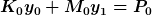
\includegraphics{../pics/8.png}\\
	Переходим к новым координатам:\\
	\begin{align*}
	z = \frac{1}{a} \arctan (y)
	\end{align*}\\
	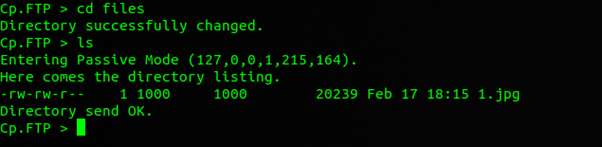
\includegraphics{../pics/9.png}\\
	\begin{align*}
	&z = \frac{1}{a} \arctan (x y_{max})\\
	&a = \dfrac{\pi}{2} - \delta, \quad y_{max} = \tan (a)
	\end{align*}\\
	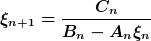
\includegraphics{../pics/10.png}\\
	Введя неравномерную сетку, запишем исходную систему в новых координатах:\\
	\begin{align*}
	&\dfrac{d}{dz} = \dfrac{d}{dx} \dfrac{d}{dz} = \dfrac{d}{dz\dfrac{dz}{dx}}\\
	&\dfrac{dz}{dx} = \dfrac{y_max}{a(1+x^2 y^2_{max})}\\
	& \dfrac{d}{dz} = \dfrac{d}{dx} \dfrac{a}{y_{max}} \left( 1 + x^2 y^2_{max} \right) = \frac{d}{dx} \tilde{p}\\
	&\tilde{p} = \frac{a}{y_{max}} \left( 1 + x^2 y^2_{max}\right)\\
	&zdz = z \frac{dz}{dx}dx = z \frac{dx}{\tilde{p}}
	\end{align*}\\
	Построение разностной схемы:
	\begin{align*}
	\omega_h = \{x_n : x_n = nh, n = \overline{1, N}, h = 1/N \}
	\end{align*}
	\begin{align*}
	\begin{cases}
	F = - \dfrac{1}{R}\dfrac{c}{3k(x)R} \dfrac{d u}{dx}\tilde{p}\\
	\dfrac{1}{R}\dfrac{1}{z} \dfrac{d}{dx}(zF)\tilde{p}=c k(x) (u_p(x) - u)\\
	x = z = 0, \quad \dfrac{du}{dx} = 0 \\
	x = z = 1, \quad F = m \dfrac{cu}{2}
	\end{cases}
	\end{align*}
	\section{Метод прогонки для реализации разностных схем с краевыми условиями 3-го рода.}
	Для примера возьмем уравнение:\\
	\begin{align*}
	\begin{cases}
	F = - \dfrac{1}{R}\dfrac{c}{3k(x)R} \dfrac{d u}{dx}\tilde{p}\\
	\dfrac{1}{R}\dfrac{1}{z} \dfrac{d}{dx}(zF)\tilde{p}=c k(x) (u_p(x) - u)\\
	x = z = 0, \quad \dfrac{du}{dx} = 0 \\
	x = z = 1, \quad F = m \dfrac{cu}{2}
	\end{cases}
	\end{align*}
	\begin{align*}
	{}
	\end{align*}
	... ПРиводим к виду: каноническая форма СЛАУ  трехдиагональной матрицей\\
	\begin{align*}
	A_n u_{n-1} - B_n u_n + D_n u_{n+1} = -E_n (5)
	\end{align*}
	где
	\begin{align*}
	&A_n = \frac{z_{n-1/2}}{k_{n-1/2}(z_n -z_{n-1})}\\
	&D_n = \frac{z_{n+1/2}}{k_{n+1/2}(z_{n+1} -z_n)}\\
	&B_n = A_n + D_n + 3R^2 k_n V_n\\
	&V_n = z_n (z_{n+1/2} - z_{n-1/2})\\
	&E_n = 3R^2 k_n V_n u_{p_n}
	\end{align*}
	Условие устойчивости прогонки 
	$|B_n| > |A_n| + |D_n|$\\
	Получим уравнения для внутренних узлов $1<=n <= N-1$.\\
	Получим краевые условия.\\
	Для замыкания (5) надо проаппроксимировать уравнения в т.0 и N . Для этого составляются разностные аналоги при x = 0(узлы 0 и 1/2) и x = N (узлы N-1/2 и N). \\
	Для x = 0 получим выражение вида $K_0 U_0 + M_0 U_1 = P_0$ (6)\\
	Для x = N получим выражение вида $K_N U_N + M_N U_{N-1} = P_N$ (7) \\
	К системе уравнений 5, 6, 7 применяем метод прогонки. \\
	Таким образом,получим систему разностных уравнений (5 6 7), приготовленную для программной реализации. Метод прогонки: в прямом мходе ищутся прогоночные коэффициент. Начальное значение прогочных коэффициентов определяются из 6 и формулы $u_n = \xi_{n+1} u_{n+1} + \eta_{n+1}$. В обратном ходе определяются функция u. $U_N$ находистя из 7 и выражения $u_{N-1} = \xi_N u_N + \eta_N$
	\section{Краевая задача для ОДУ. Методы решения квазилинейных разностных схем для уравнения 2-го порядка (простые итерации и метод Ньютона).}
	Пример нелинейного уравнения
	\begin{align*}
	\frac{\partial}{\partial x}\left( \lambda(T) \frac{\partial T}{\partial x}  \right) + q(T) = 0
	\end{align*}
	Простая аппроксимация 
	\begin{align*}
	A_n y_{n-1} - B_n y_n + C-n y_{n+1} = -F_n
	\end{align*}
	уравнение квализейны\\
	\begin{align*}
	&A_n = \chi_{n-1/2} \\
	&C_n = \chi_{n+1/2} \\
	&B_n = A_n + C_n + 3R^2 \lambda_n V_n \\
	&V_n = z_n (z_{n+1/2} - z_{n-1/2})\\
	&F_n = 3R^2 \lambda_n V_n U_{p_n}\\\\
	&A_n(y_{n-1}, y_n)y_{n-1} - B_n(y_{n-1}, y_n, y_{n+1})y_n + C_n(y_n, y_{n+1})y_{n+1} = -F_n
	\end{align*}
	Методы решений квазилинейных уравнений:
	\begin{enumerate}
		\item Метод простых итераций\\
		\begin{align*}
		A_n(y^{(s-1)}_{n-1}, y^{(s-1)}_n)y^{(s)}_{n-1} - B_n(y^{(s-1)}_{n-1}, y^{(s-1)}_n, y^{(s-1)}_{n+1})y^{(s)}_n + C_n(y^{(s-1)}_n, y^{(s-1)}_{n+1})y^{(s)}_{n+1} = -F^{(s-1)}_n
		\end{align*}
		Окончание итерации 
		\begin{align*}
		max \Bigl| \frac{T^{}_n - T^{}_n}{T^{}_n} \Bigl | < \varepsilon
		\end{align*}
		абсолютно точное моделирование : \\
		\begin{align*}
		C_p \frac{\partial T}{\partial t} = \frac{\partial}{\partial r}\left( \lambda(T) \frac{\partial T}{\partial x} + y(T) \right)
		\end{align*}
		\item Метод Ньютона\\
		Линеаризуем систему $f(x_1, x_2, x_3) = 0 : f(x^{(s)}_1, x^{(s)}_2, x^{(s)}_3) + \sum_{k=1}^{3} \dfrac{\partial f}{\partial x_k}(x^{(s+1)}_k - x^{(s)}_k) = 0$ \\
		$\Rightarrow$ $\sum_{k=1}^{3} \dfrac{\partial f^{(s)}}{\partial x_k} \triangle x^{(s)}_k = -f(x^{(s)}_1, x^{(s)}_2, x^{(s)}_3)$\\
		$x^{(s+1)}_k = x^{(s)}_k + \triangle x^{(s)}_k$, где $f = f_m()$
		\begin{align*}
		&\left[ \frac{\partial A_n}{\partial y_{n-1}} y_{n-1} + A^{(s)}_n + \frac{\partial B_n}{\partial y_{n-1}} y_n \right]^{(s)}\triangle y^{(s)}_{n-1} \\
		- &\left[ \frac{\partial A_n}{\partial y_{n}} y_{n-1} - \frac{\partial B_n}{\partial y_{n}} y_n - B_n + \frac{\partial C_n}{\partial y_n} \right]^{(s)}\triangle y^{(s)}_{n} \\
		- &\left[ \frac{\partial B_n}{\partial y_{n+1}} y_{n} - \frac{\partial C_n}{\partial y_{n+1}} y_{n+1} + C_n  \right]^{(s)}\triangle y^{(s)}_{n+1} = -F_n
		\end{align*}
		Методом прогонки, пока не станет $\Bigl| \dfrac{\triangle y^{(s)}_n}{\triangle y^{(s+1)}_n} \Bigl| < \varepsilon$\\
	\end{enumerate}
	\section{Уравнения в частных производных. Области применения. Классификация уравнений второго порядка. Общие понятия о методах решения.}
	Уравнения в частных производных - уравнение, которое содержит боле чем одну независимую переменную. Эти муравнения описывают поля: скоростей, гравитации, температур, концентрации в-в, радиационные поля, электромагнитные. Независимыми переменными являются время и 3 декартовы координаты. Уравнение задаетяс в некоторой области.\\
	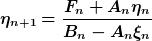
\includegraphics{../pics/11.png}\\
	Классификация:\\
	Мы в  нашем курсе рассматриваем уравнения , линейные относительно старших производных. Применительно к двум переменным, общий вид уравнения следующий:\\
	\begin{align*}
	a_{11}u_{xx} + 2a_{12}u_{xy} + a_{22}u_{yy} + F(x, y, u, u_x, u_y) = 0
	\end{align*}
	x,y - независимые переменные. \\
	u(x, y) - искомая функция\\
	\begin{align*}
	u_{xx} = \frac{\partial^2 u}{\partial x^2}\\
	u_{x} = \frac{\partial u}{\partial x}\\
	u_{xy} = \frac{\partial^2 u}{\partial x \partial y}\\
	\end{align*}
	\begin{enumerate}
		\item Если $a_{11}, a_{12}, a_{22}$ зависят от $x,y,u,u_x,u_y$ (или хотя от одного из них) , то уравнение называется квазилинейным.
		\item Если $a_{11}, a_{12}, a_{22}$ не зависят от $u,u_x,u_y$ но зависят от x,y, то уравнение называется линейным относительно старших производных.
		\item  Уравнение вида $a_{11}u_{xx} + 2a_{12}u_{xy} + a_{22}u_{yy} + bu_x + cu_y + du + f(x,y) = 0$, где $a_{ij} = a_{ij}(x,y)$\\
		b,c,d зависят толькот x,y, то уравнение называется линейным
		\item Все коэффициеты константы - уравнение называется линейным с постоянными коэффициентами (самый простой тип).
	\end{enumerate}
	Чтобы отличить типы уравнений (и соотв способ решения) вводится дискриминант
	$d = a^2_{12} - a_{11}a_{22}$
	\begin{enumerate}
		\item d > 0 - гиперболическое
		\item d = 0 - параболическое
		\item d < 0 - эллиптическое
	\end{enumerate}
	\begin{align*}
	&\frac{\partial^2 u}{\partial t^2} = a \frac{\partial^2 u}{\partial x^2} + f(x,t) - \quad \text{гиперболическое}\\
	&\frac{\partial^2 u}{\partial x^2} + \frac{\partial^2 u}{\partial y^2} + f(x,y) = 0 \quad \text{эллиптическое}\\
	&\frac{\partial u }{\partial t}  = a \frac{\partial^2 u}{\partial x^2} + f(x,t) \quad \text{параболическое}
	\end{align*}
	Метод установления - решааем нестационарную задачу, пока время не установится в ноль. Например, приняем матричную прогонку. Увеличивается время счета, но уравнения сводтся к более простому типу. \\
	Методы решения:
	\begin{enumerate}
		\item Точные аналитические (метод разделения переменных, метод бегущих волн, метод функции источника (Грина))
		\item Приближенные аналитические (метод Бубнова-Галеркина, мето малого параметра)
		\item Численные (сеточный(разностный) метод, проекционно-сеточный (метод конечных элементов))
	\end{enumerate}
	\section{Уравнения в частных производных. Постановка задач Коши, краевых  и смешанных краевых задач. Привести примеры с краевыми условиями 1-го, 2-го и 3-го родов.}
	Уравнения в частных производных - уравнение, которое содержит боле чем одну независимую переменную.  Независимыми переменными являются время и 3 декартовы координаты. Уравнение задаетяс в некоторой области.\\
	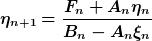
\includegraphics{../pics/11.png}\\\\
	Задача может быть сформулирована как задача Коши (есть нач условия , нет граничных условий) в бесконечном пространстве G, или как чисто краевая (стционарная) задача (времени нет), или как смешанная краевая задача. (нестационарная задача). 
	Пример смешанной краевой задачи:\\
	Единственное решение выделяется заданием начальных условий. Например, при t = 0 \\
	$u(\vec{r}, 0) = \mu(\vec{F})$\\
	И граничных условий $u(\vec{r}, 0) \Bigl|_{\varGamma} = \mu_1 (\vec{r}, t)$, где $\varGamma$ - граница G\\\\
	Пример 1: уравнение параболического типа в одномерном варианте (линейный случай с пост коэффициентами):\\
	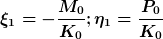
\includegraphics{../pics/12.png}
	\begin{align*}
	&\frac{\partial u }{\partial t} = a \frac{\partial^2 u}{\partial x^2} + f(x,t)\\
	&\text{н.у. } u(x,0) = \mu(x)\\
	\end{align*}
	\begin{align*}
	\text{гр.у. 1-го рода } \quad &u(a, t) = \mu_1(t)\\
	&u(b,t) = \mu_2(t)\\
	\text{гр.у. 2-го рода } \quad &\frac{\partial u}{\partial x} \Bigl|_{x=a} = \alpha(t)\\
	\text{гр.у. 3-го рода } \quad &\alpha \frac{\partial u}{\partial x} \Bigl|_{x=a} + \beta u(a, t) = \psi(t)\\
	\end{align*}
	Левое и правое г.у. могут быть разных родов.\\\\
	Пример 2: уравнение параболического типа в двумерном варианте\\
	\begin{align*}
	\frac{\partial u }{\partial t}  = a \frac{\partial^2 u}{\partial x^2} + a \frac{\partial^2 u}{\partial y^2} + f(x,y,t)
	\end{align*}\\
	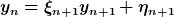
\includegraphics{../pics/13.png}\\
	Решение ищется в прямоугольной области [a, b]. Если область не прямоугольная - проблемы.\\
	\begin{align*}
	\text{н.у. }&:u(x,y,0) = \mu(x,y)\\
	\text{г.у. }&:\\
	\end{align*}\\
	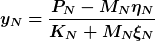
\includegraphics{../pics/14.png}\\
	\begin{align*}
	&u(0,y,t) = \mu_1(y,t)\\
	&u(a,y,t) = \mu_2(y,t)\\
	&u(x,0,t) = \mu_3(x,t)\\
	&u(x,b,t) = \mu_4(x,t)\\
	\end{align*}
	\section{Уравнения в частных производных с постоянными коэффициентами. Основные понятия метода конечных разностей. Понятие о явных и неявных схемах. }
	Пример уравнения параболического типа с постоянными коэффициентами:\\
	\begin{align*}
	\frac{\partial u }{\partial t}  &= a \frac{\partial^2 u}{\partial x^2} + f(x,t)\\
	u(x,0) &= \mu(x)\\
	\mu(a, t) &= \mu_1(t)\\
	\mu(b, t) &= \mu_2(t)
	\end{align*}
	В пространстве вводится сетка - множество узлов, которые образуются в результате пересечений параллельных t и x прямых. \\
	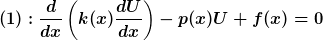
\includegraphics{../pics/15.png}
	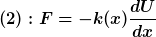
\includegraphics{../pics/16.png}\\\\
	Сетка:
	\begin{align*}
	&\omega_{h \tau} = \{ x_n = a + nh, t_m = m\tau, n = \overline{0, N}, m = \overline{0, M} \}\\
	&u(x_n, t_m) = u^m_n\\
	&u(x_n, t_{m+1}) = u^{m+1}_n
	\end{align*}
	Будем обозначать \\
	\begin{align*}
	&u^m_n = u_n\\
	&u^{m+1}_n = \hat{u_n}
	\end{align*}
	u - точное решение, которое не можем посчитать\\
	y - разностное решение(приближенное)\\
	\begin{align*}
	&y^m_n = y_n\\
	&y^{m+1}_n = \hat{y_n}
	\end{align*}
	Производную заменяем разностью:\\
	\begin{align*}
	\frac{y^{m+1}_n - y^m_n}{\tau} = \frac{\hat{y_n} - y_n}{\tau}
	\end{align*}
	На сетке совокупность узлов, относящихся к фикс моменту времени, образуют слой. \\
	Дискретные значения функции в узлах образуют сеточную фнукцию. Результат приближенного решения будем обозначать $y_n$ и $\hat{y_n}$\\
	Для составления простейшей разностной схемы (методом разностной аппроксимации) необходимо на сетке выбрать шаблок,то есть конфигурацию узлов, на котрой производные будут заменены их разностными аналогами. \\
	Разностная схема имеет вид:\\
	\begin{enumerate}
		\item 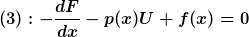
\includegraphics{../pics/17.png}\\
		\begin{align*}
		&\frac{\hat{y_n} - y_n}{\tau} = a \frac{\hat{y_{n-1}} - 2\hat{y_n} + \hat{y_{n+1}} }{h^2} + f(x_n, t_{m+1})\\
		&t=0, \quad y_n = \mu(x_n)\\
		&x=a, \quad \hat{y_0} = \mu_1(t_{m+1})\\
		&x=b, \quad \hat{y_N} = \mu_2(t_{m+1})\\
		\end{align*}
		\item 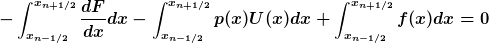
\includegraphics{../pics/18.png}\\
		\begin{align*}
		&\frac{\hat{y_n} - y_n}{\tau} = a \frac{y_{n-1} - 2y_n + y_{n+1} }{h^2} + f(x_n, t_m)\\
		&t=0, \quad y_n = \mu(x_n)\\
		&x=a, \quad \hat{y_0} = \mu_1(t_{m})\\
		&x=b, \quad \hat{y_N} = \mu_2(t_{m})\\
		\end{align*}
		\item 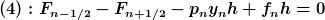
\includegraphics{../pics/19.png}\\
		\begin{align*}
		&\frac{\hat{y_n} - y_n}{\tau} = a G \frac{\hat{y_{n-1}} - 2\hat{y_n} + \hat{y_{n+1}} }{h^2} + a(1-G) \frac{y_{n-1} - 2y_n + y_{n+1} }{h^2}+\varphi \\
		&t=0, \quad y_n = \mu(x_n)\\
		&x=a, \quad \hat{y_0} = \mu_1(t_{m+1})\\
		&x=b, \quad \hat{y_N} = \mu_2(t_{m+1})\\
		\end{align*}
	\end{enumerate}
	Первая схема неявная, чтобы найти $\hat{y}$ нужно решить систему уравнений. Схема два явная - обычная формула. Схема три при G = 1 выходит в 1, при G = 0 в 2. В явной схеме устойчивость зависит от шага, неявная схема абсолютно устойчива. В 3 схеме при G = 1/2 повышаем точность аппроксимации, но теряется устойчивость. На G накладываются ограничения. 
	\section{Квазилинейные уравнения в частных производных. Получение разностной схемы для одномерного параболического уравнения с краевыми условиями 3-го рода интегро- интерполяционным методом.}
	Если коэффициенты $a_{11}, a_{12}, a_{22}$ зависят от $x,y,u,u_x,u_y$ (или хотя от одного из них) , то уравнение называется квазилинейным.\\
	\begin{align*}
	c(u) \frac{\partial u}{\partial t} = \frac{\partial}{\partial x}\left( \lambda(u)\frac{\partial u}{\partial x} \right) + f(u)
	\end{align*}
	Чтобы применить ИИМ , нужно выбрать шаблон. Построим чисто неявную схему. Шаблон:\\
	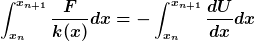
\includegraphics{../pics/20.png}\\
	Введем понятие потока:\\
	\begin{align*}
	\begin{cases}
	F = -a \frac{\partial u}{\partial x} \quad (1)\\
	c(u) = \frac{\partial u}{\partial t} = -\frac{\partial F}{\partial x} + f(u) \quad (2)
	\end{cases}
	\end{align*}
	\begin{align*}
	\int_{x_{n-1/2}}^{x_{n+1/2}}dx\int_{t_m}^{t_{m+\tau}} c(u) \frac{\partial u}{\partial t}dt =  -\int_{t_m}^{t_{m+\tau}} dt \int_{x_{n-1/2}}^{x_{n+1/2}}\frac{\partial F}{\partial x}dx + \int_{t_m}^{t_{m+1}}\int_{x_{n-1/2}}^{x_{n+1/2}}f(x,t) dx dt
	\end{align*}	
	В общем виде:
	\begin{align*}
	\int_{V}div \vec{F} dV = \int_{\sum} \vec{F} \vec{n} d\sum
	\end{align*}

	\begin{align*}
	\int_{x_{n-1/2}}^{x_{n+1/2}} dx \hat{c}(\hat{u} - u) = \int_{t_m}^{t_{m+1}} (F_{n-1/2} - F_{n+1/2})dt + f(x_n, t_{m+1})\tau h 
	\end{align*}
	последнее слагаемое из метода средних\\
	$\hat{c}$ заменим $c(t_{m+1})$ и  получаем порядок точности O(1)\\
	\begin{align*}
	\hat{c_n}(\hat{y_n} - y_n) h = (\hat{F_{n-1/2}} - \hat{F_{n+1/2}}) \tau + f(x_n, t_{m+1}) \tau h
	\end{align*}
	Проинтегрируем (1) и избавимся  от потока:\\
	\begin{align*}
	&\int_{x_n}^{x_{n+1}}\frac{F}{\lambda}dx = -\int_{x_n}^{x_{n+1}}\frac{\partial u}{\partial x} dx\\
	&F_{n+1/2}\int_{x_n}^{x_{n+1}}\frac{\partial x}{\lambda} = y_n - y_{n+1}\\
	&F_{n+1/2} = \chi_{n+1/2}\frac{y_n - y_{n+1}}{h}\\
	&\chi_{n+1/2} = \frac{\lambda_n + \lambda_{n+1}}{2}	
	\end{align*}
	Применительно к решаемой задаче:\\
	\begin{align*}
	&\hat{F}_{n+1/2} = \hat{\chi}_{n+1/2}\frac{\hat{y}_n - \hat{y}_{n+1}}{h}\\
	&\hat{F}_{n-1/2} = \hat{\chi}_{n-1/2}\frac{\hat{y}_{n-1} - \hat{y}_{n}}{h}\\\\
	&\hat{A}_n\hat{y}_{n-1} - \hat{B}_n \hat{y}_n + \hat{C}_n \hat{y}_{n+1} = -\hat{F}_n
	\end{align*}	
	квазилинейная разостная схема с трехдиагональой матрицей (решаем методом итераций).
	\section{Решение разностных схем для квазилинейных уравнений в частных производных- метод простых итераций и метод Ньютона.}
		\begin{enumerate}
		\item Метод простых итераций\\
		\begin{align*}
		&A^{(s-1)}_n y^{(s)}_{n-1} - B^{(s-1)}_n y^{(s)}_n + C^{(s-1)}_n y^{(s)}_{n+1} = -F^{(s-1)}_n\\
		&K^{(s-1)}_0 \hat{y}^{(s)}_0 + M^{(s-1)}_0 \hat{y}^{(s)}_1 = P^{(s-1)}_1\\
		&K^{(s-1)}_N \hat{y}^{(s)}_N + M^{(s-1)}_N \hat{y}^{(s)}_{N-1} = P^{(s-1)}_N\\
		\end{align*}
		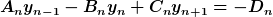
\includegraphics{../pics/21.png}
		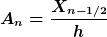
\includegraphics{../pics/22.png}\\\\
		Нестационарный процесс:\\
		\begin{align*}
		&c\frac{\partial T}{\partial T} = \frac{\partial}{\partial x}\left( d \frac{\partial T}{\partial x} \right) + f(T)\\
		&\frac{\partial}{\partial x}\left( \lambda \frac{\partial T}{\partial x}  \right)	+ f(T)
		\end{align*}
		Сходимость метода простхы тераций не очеивдна. Влиять на сходимость можно изменяя $\tau$. Есть другой пример (метод релаксации).\\
		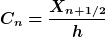
\includegraphics{../pics/23.png}\\
		Все коэффициенты $(A^{(s-1)}_n, B_n, C_n, D_n, K_0, F_N)$\\
		\begin{align*}
		&y^{\zeta} = y + \xi(y^{(s)} - y)\\
		&\xi = 0,2 .. 0,9\\
		& max \Bigl| \frac{y^{\xi}_n - y^{(s)}_n}{y^{(s)}_n} \Bigl|<= \xi
		\end{align*}
		\item Линеаризация разностной схемы методом Ньютона

		\begin{align*}
		&\hat{A}_n = \hat{A}_n(\hat{y}_{n-1}, \hat{y}_n)\\
		&\hat{B}_n = \hat{B}_n(\hat{y}_{n+1}, \hat{y}_n, \hat{y}_{n+1})\\
		&\hat{C}_n = \hat{C}_n(\hat{y}_{n}, \hat{y}_{n+1})\\
		&\hat{F}_n = \hat{F}_n(\hat{y}_n)\\\\
		&\text{Тут все с крышками}\\		
		&\left[ \frac{\partial A_n}{\partial y_{n-1}} y_{n-1} + A_n + \frac{\partial B_n}{\partial y_{n-1}} y_n \right]\triangle y_{n-1} \\
		- &\left[ \frac{\partial A_n}{\partial y_{n}} y_{n-1} - \frac{\partial B_n}{\partial y_{n}} y_n - B_n + \frac{\partial C_n}{\partial y_n} \right]\triangle y_{n} \\
		- &\left[ \frac{\partial B_n}{\partial y_{n+1}} y_{n} - \frac{\partial C_n}{\partial y_{n+1}} y_{n+1} + C_n  \right]\triangle y_{n+1} = -\frac{\partial F}{\partial y_n} \Bigl|_{(s-1)} \triangle \hat{y}_n \\
		&= -\left( A_n y_{n-1} - B_n y_n + C_n y_{n+1} + F_n \right) \Bigl|_{(s-1)}\\\\
		&\triangle \hat{y}^{(s)}_n , \quad n = \overline{1, N-1}\\
		&\hat{y}^{(s)}_n = y^{(s-1)}_n + \triangle y^{(s)}_n
		\end{align*}
		
	\end{enumerate}

	\section{Методы повышения порядка аппроксимации краевых условий 2-го и 3-го родов (интегро- интерполяционная процедура, разложение в ряд Тейлора, введение фиктивного узла).}	
	\begin{align*}
	&c\frac{\partial u}{\partial t} = a \frac{\partial^2 u}{\partial x^2} + f(x, t)\\
	& x = 0, \quad \frac{\partial u}{\partial x} = \mu(t) 
	\end{align*}
	\begin{enumerate}
		\item Интегро-интерполяционный метод\\
		\begin{align*}
		&\int_{t}^{t+\tau} \int_{0}^{x_{1/2}} c \frac{\partial u}{\partial t} dt dx = - \int_{t}^{t+\tau} dt \int_{0}^{x_{1/2}}\frac{\partial F}{\partial x} dx + \int_{t}^{t+\tau} \int_{0}^{x_{1/2}} f(x, t)dx dt\\
		&F_0 = -a \mu(t)\\
		& F_{1/2} = \chi_{1/2}\frac{y_1 - y_0}{h}
		\end{align*}
		\item Разложение в ряд Тейлора \\
		\begin{align*}
		&u_1 = u_0 + h\frac{\partial u}{\partial x} + \frac{h^2}{2!} \frac{\partial^ u}{\partial x^2 }+...\\
		&\frac{\partial u}{\partial x} = \mu(t)\\
		&\frac{\partial^2 u}{\partial x^2 }= \frac{c}{a}\frac{\partial u}{\partial t} - \frac{f}{a}\\
		&y_1 = \hat{y}_0 + h\mu(t)_{m+1} + \frac{h^2}{2}\left( \frac{c}{a}\frac{\partial u}{\partial t} - \frac{f}{a} \right)\\
		&y_1 = \hat{y}_0 + h\mu(t)_{m+1} + \frac{h^2}{2}\left( \frac{c}{a}\frac{ \hat{y}_0 - y_0}{\tau} - \frac{f}{a}\right)\\
		\end{align*}
		\item Введение фиктивного узла(-1 и 1)\\
		Краевое условие\\
		\begin{align*}
		&\frac{\hat{y}_1 - \hat{y}_{-1}}{2h} = \mu(t)_{m+1} \rightarrow \hat{y}_{-1} = \hat{y}_1 - 2h \mu(t_{m+1})\\
		&A_0 \hat{y}_{-1} - B_0 \hat{y}_0 + C_0 \hat{y}_1 = -F_0 \quad \text{исключают} \hat{y}_{-1} \text{с помощью (1)}\\
		&M_0 \hat{y}_0 + Q_0 \hat{y}_1 = \varGamma_0
		\end{align*}
	\end{enumerate}
	\section{Понятие невязки для разностных схем. Привести пример вычисления невязки для неявной схемы.}	
	Невязка\\
	\begin{align*}
	\frac{\partial u}{\partial t} = a \frac{\partial^2 u}{\partial x^2} + f(x,t)
	\end{align*}
	Разностная схема \\
	\begin{align*}
	&\frac{\hat{y}_n - y_n}{\tau} = a \frac{y_{n-1} - 2y_n + y_{n+1}}{h^2} + f(x_n, t_n) \quad \longrightarrow A_n y = \varphi_n\\
	&\psi_n = \varphi_n - A_n u = (Au - f)-(A-nu-\varphi_n)
	\end{align*}
	Невязка отражает в какой мере разностная схема соответствует дифф уравнению. \\
	Сходимость означает, что при $h\rightarrow 0$ y переходит в u. \\
	Два свойства разностных схем: аппроксимация и устойчивость.\\
	Найдем невязку для ДУ и составим разностную схему. Невязка ищется разложением в ряды Тейлора.\\
	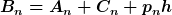
\includegraphics{../pics/24.png}\\
	\begin{align*}
	&\psi_n = \frac{\partial u}{\partial t} - a \frac{\partial^2 u}{\partial x^2} - f (x,t) - \left[ \frac{\hat{u}_n - u_n}{\tau} - \frac{a}{h^2} (u_{n-1} - 2u_n + u_{n+1})-f(x_n, t_m)\right]\\
	&\hat{u}_n = u_n + \tau  \frac{\partial u}{\partial t} + \frac{\tau^2}{2!} \frac{\partial^2 u}{\partial t^2} \Bigl|_{x_n, \theta_m, t_m} <= \theta_m <= t_{m+1}\\
	&u_{n\pm 1} = u_n  \pm h \frac{\partial u}{\partial x} + \frac{h^2}{2!} \frac{\partial^2 u}{\partial x^2} \pm \frac{h^3}{3!} \frac{\partial^3 u}{\partial x^3}  + \frac{h^4}{4!} \frac{\partial^4 u}{\partial x^4} \Bigl|_{\xi_{n\pm 1}, t_m}\\
	&x_{n-1} <= \xi_{n-1} <= x_n\\
	&x_n <= \xi_{n+1} <= x_{n+1}\\\\
	&\psi_n = \left( \frac{\partial u}{\partial t} - a \frac{\partial^2 u}{\partial x^2} + f (x,t) \right)\Bigl|_{x_m, t_m} - \left[ \frac{\partial u}{\partial t} + \frac{\tau}{2}\frac{\partial^2 u}{\partial t^2}\Bigl|_{x_n, \theta_m} - \frac{a}{h^2} \left( h^2 \frac{\partial^2 u}{\partial x^2} +  \frac{h^4}{12} \frac{\partial^4 u}{\partial x^4} \Bigl|_{x_n, \xi_{n \pm 1}}  -f(x_n, t_m) \right) \right]\ = \\
	& -\frac{\tau}{2} \frac{\partial^2 u}{\partial t^2} \Bigl|_{x_n, \theta_m} + \frac{a h^2}{12}\frac{\partial^4 u}{\partial x^4} = O(\tau + h^2)
	\end{align*}
	то есть  $|\psi_n| \rightarrow 0$, если $h \rightarrow 0 , \tau \rightarrow 0$ со скоростью $\tau$ (первый порядок аппроксимаци) и $h^2$ (вторым порядком аппроксимации).
	\section{Свойство аппроксимации разностных схем для уравнений в частных производных.}
	Аппроксимация\\
	\begin{align*}
	&Au = f\\
	&Bu = \beta
	\end{align*}
	\begin{align*}
	&\frac{\partial u}{\partial t} = a \frac{\partial^2 u}{\partial x^2} + f(x,t)\\
	&\begin{cases}
	x = 0, \quad \dfrac{\partial u}{\partial x} = \alpha(u - y)\\
	x = l, \quad \dfrac{\partial u}{\partial x} = \eta(u - \xi)\\
	t = 0, \quad u(x, 0) = \mu(x)
	\end{cases}
	\end{align*}	
	Разностная схема
	\begin{align*}
	&A_n u = f_n\\
	&B_n u = \beta_n
	\end{align*}
	\begin{align*}
	&\frac{\hat{y}_n - y_n}{\tau} = \frac{a}{h^2}(\hat{y}_{n-1} -2\hat{y}_n + \hat{y}_{n+1}) + f_n\\
	&\frac{\hat{y}_1 - \hat{y}_0}{h} = \alpha(\hat{y}_0 - j)\\
	&\frac{\hat{y}_N - \hat{y}_{N-1}}{h} = \eta (\hat{y}_N - \xi)
	\end{align*}
	Невязка
	\begin{align*}
	\psi_n = (A_n u - f_n) + (Au - f)\\
	\rho_n =(Bu - \beta) + (B_n u - \beta_n)
	\end{align*}
	Разностная схема аппроксимирует исходную диф задачу , если \\
	$||\psi_n||\rightarrow0, \quad ||\rho_n || \rightarrow 0$ при $h \rightarrow 0, \tau \rightarrow 0$\\
	Разностная схема аппроксимирует исходную диф задачу с порядкм k и p , если\\
	$||\psi_n|| = O(\tau^k + h^p)$\\
	$||\rho_n || = O(\tau^k + h^p)$ при $h \rightarrow 0, \tau \rightarrow 0$ \\
	c k-ым порядком по вреени и p-ым по координате.\\
	Это безусловная аппроксимация ($h \rightarrow 0, \tau \rightarrow 0$ независимо).\\\\
	При условной аппроксимации \\
	$||\psi_n|| = O(\tau^k + h^p + \frac{r^m}{h^q})$\\
	$||\rho_n || = O(\tau^k + h^p + \frac{r^m}{h^q})$\\
	$h \rightarrow 0, \quad \tau \rightarrow 0,\quad\frac{r^m}{h^q} \rightarrow 0 $\\
	Если например выбрать $\tau = h ^{q/m}$ то аппроксимации не будет(наше уравнение не будет аппроксимировать исходное ДУ ).\\
	Если невязка $\rightarrow 0$ , то разностная схема переходит в исходный ДУ . НЕвязка показывает близость двух типов уравнений(исходное и разностное). Из аппроксимации и устойчивости следует сходимость. 
	\section{Понятие устойчивости разностных схем по начальным данным и правой части. На основе принципа максимума исследовать устойчивость явной и неявной схем для уравне-ния параболического типа.}	
	Устойчивость - непрерывная зависимость решения от входных данных . Это означает, что малые изменения входных данных должны приводить к малому изменению результата. \\
	Устойчивость по начальным данным означает насколько чувствительна разностная схема к изменению начальных условий. \\
	Два метода определения устойчивости:
	\begin{enumerate}
		\item Принцип максимума\\
		Запишем разностную схему в следующем виде:\\
		\begin{align*}
		&\sum_{k}a_k \hat{y}_{n+k} = \sum_{p} b_p y_{n+p} + \rho_n\\
		&|a_0| = max(a_k)
		\end{align*}
		Схема устойчива по начальным данным, если $(1+c\tau)|a_0|>= \sum_{k\neq 0}|a_k|+\sum_{p}|b_p|$\\
		Схема устойчива по правой части, если справедливо утверждение выше и $|a_0| - \sum_{k \neq 0}|a_k| >= \frac{D}{\tau}, 0< D = const$\\
		Применительно к нашей схеме:
		\begin{align*}
		a_{-1} = \frac{a}{h^2}, \quad a_0 = \frac{2a}{h^2} + \frac{1}{\tau} , |a_1| = \frac{a}{h^2}
		\end{align*}
		Аналогично работаем с краевыми условиями\\
		Коэффициентный анализ показывает, что выписанная разностная схема устойчива по правой части во всех внутренних узлах и устойчива по начальным данным во всех узлах.
		\item Метод разделения переменных \\
		Проверяется устойчивость по начальным данным\\
		$z_n = y_n - u_n$ - погрешность\\
		Считаем,что разностная схема аппроксимирует задачу. Невязка стремится к нулю, Правая часть (ф-ция f) имеет нулеую погрешность. Тогда \\
		\begin{align*}
		&\frac{\hat{z}_n - z_n}{\tau}  =\frac{a}{h^2} \left( \hat{z}_{n-1} - 2\hat{z}_n + \hat{z}_{n+1} \right) \quad\text{неявная схема}\\
		&\frac{\hat{z}_n - z_n}{\tau}  =\frac{a}{h^2} \left( z_{n-1} - 2z_n + z_{n+1} \right) \quad\text{явная схема}\\
		\end{align*}
		Для явной схемы \\
		\begin{align*}
		z(x_n, t_m) = z_n = \rho^m_q e^{i \pi q x_n / l}
		\end{align*}
		q - номер гармоники, $\rho$ - показатель роста гармоники\\
		Чтобы погрешность не увеличивалась условия устойчивости:\\
		$\forall q (1 + c\tau) |p_q| < 1$, c обычно = 0.\\
		Признак неустойчивости:\\
		$\exists q: |\rho_q| >1$
	\end{enumerate}
	\section{На основе метода разделения переменных исследовать устойчивость четырехточечных явной и неявной разностных схем для уравнения параболического типа.}	
	\begin{align*}
	\frac{\partial u }{\partial t}  = a \frac{\partial^2 u}{\partial x^2} + f(x,t)
	\end{align*}
	Исследуем методом разделения переменных явную разностную схему:
	\begin{align*}
	&\frac{z_n(\rho_q -1 )}{\tau} = \frac{\rho^m_q e^{i \pi q (x_n - h) / l} (p_q -1)}{\tau} = \frac{a}{h^2} ( \rho^m_q e^{i \pi q x_n / l} - 2 \rho^m_q e^{i \pi q x_n / l} + \rho^m_q e^{i \pi q (x_n + h) / l})\\
	&(p_q - 1) = \frac{\tau a }{h^2} (e^{-i \pi q h / l} - 2 + e^{+i \pi q h / l})\\
	&e^{i \varphi } = cos(\varphi) + i sin(\varphi)\\
	&e^{-i \pi q h / l}  + e^{+i \pi q h / l}	= cos(\pi q h / l) - i sin(\pi q h / l) + cos(\pi q h / l) + i sin(\pi q h / l) = 2 cos(\pi q h / l)\\
	&(p_q - 1) = \frac{2\tau a}{h^2} = (cos(\pi q h / l) - 1)\\
	&\text{или}\\
	&p_q-1 = \frac{2\tau a}{h^2} (-2 sin^2(\frac{\pi q h}{2l}))\\
	&p_q = 1 - \frac{4\tau a}{h^2} sin^2(\frac{\pi q h}{2l}) \\
	&p_q <= 1 : 1 - \frac{4\tau a}{h^2} sin^2(\frac{\pi q h}{2l}) <= 1\\
	&p_q >= - 1 : 1 - \frac{4\tau a}{h^2} sin^2(\frac{\pi q h}{2l}) >= -1\\
	&\frac{4\tau a}{h^2} <= 2, \frac{\tau}{h^2} <= \frac{1}{2a}, \tau <= \frac{h^2}{2a}	 (*)
	\end{align*}
	Разностная схма являетя условно устойчивоой, $\tau$ должно удовлетворять условиям (*). \\
	Если исходное диф уравнение квазилинейное или его коэффициенты зависят от координат, тогда этот метод не удается применить в чистом виде, и используют так называемый метод замороженных коэффициентов. 
	
	\section{На основе метода разделения переменных исследовать устойчивость шеститочечной разностной схемы для уравнения параболического типа.}	
	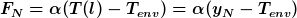
\includegraphics{../pics/37.png}\\
	\section{Уравнения в частных производных. Сходимость разностных схем. Теорема о сходимости разностного решения к точному.}	
	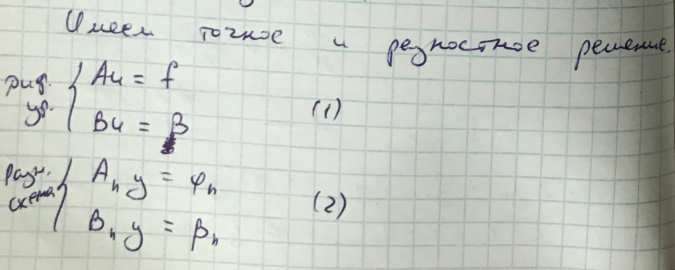
\includegraphics{../pics/38_1.png}\\\\
	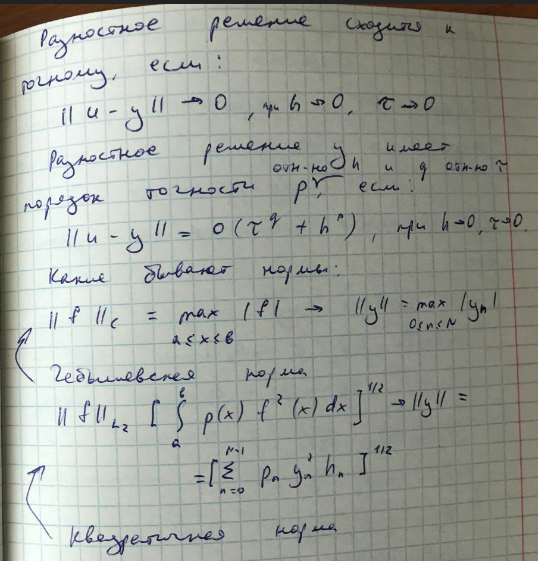
\includegraphics{../pics/38_2.png}\\\\
	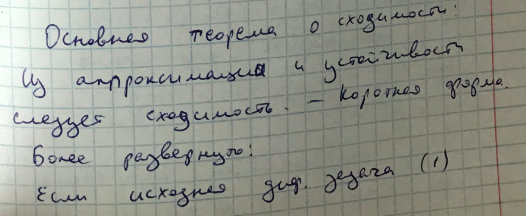
\includegraphics{../pics/38_3.png}\\\\
	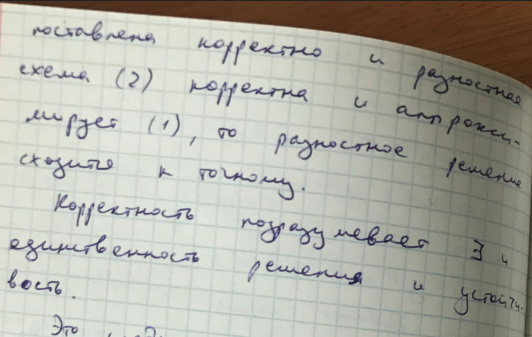
\includegraphics{../pics/38_4.png}\\\\
	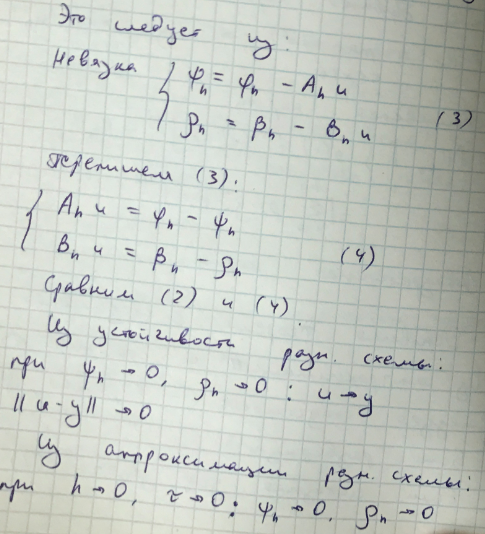
\includegraphics{../pics/38_5.png}\\\\
	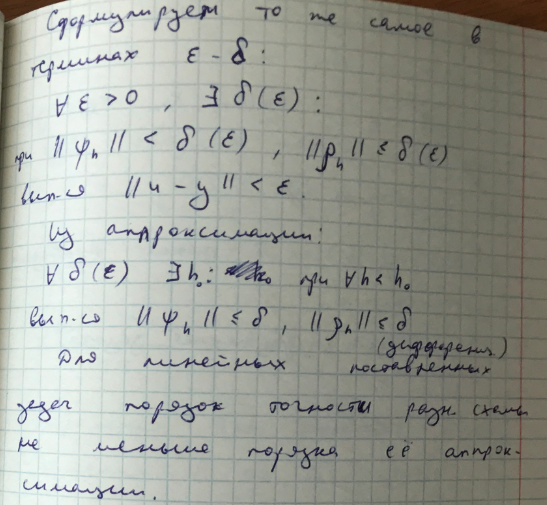
\includegraphics{../pics/38_6.png}\\\\
	\section{Метод продольно-поперечной прогонки для решения многомерных уравнений в частных производных.}	
	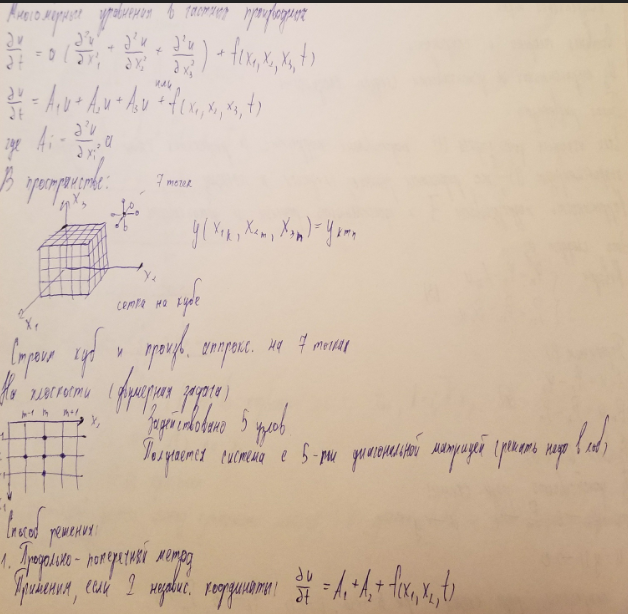
\includegraphics{../pics/39_1.png}\\\\
	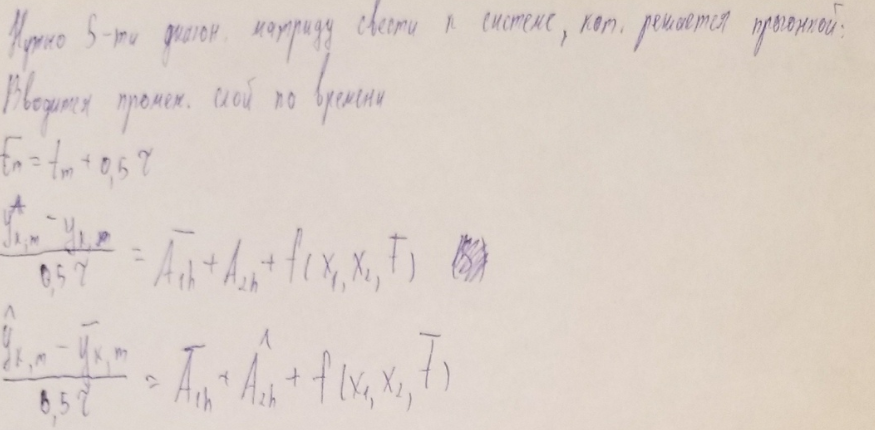
\includegraphics[width=7.0in]{../pics/39_2.png}\\\\
	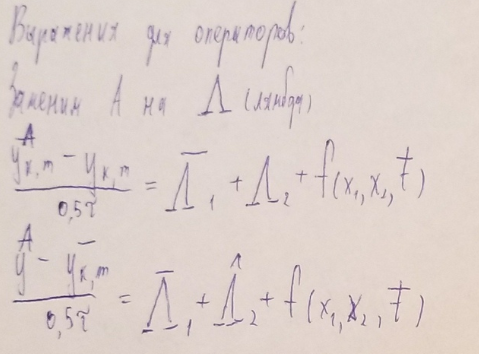
\includegraphics{../pics/39_3.png}\\\\
	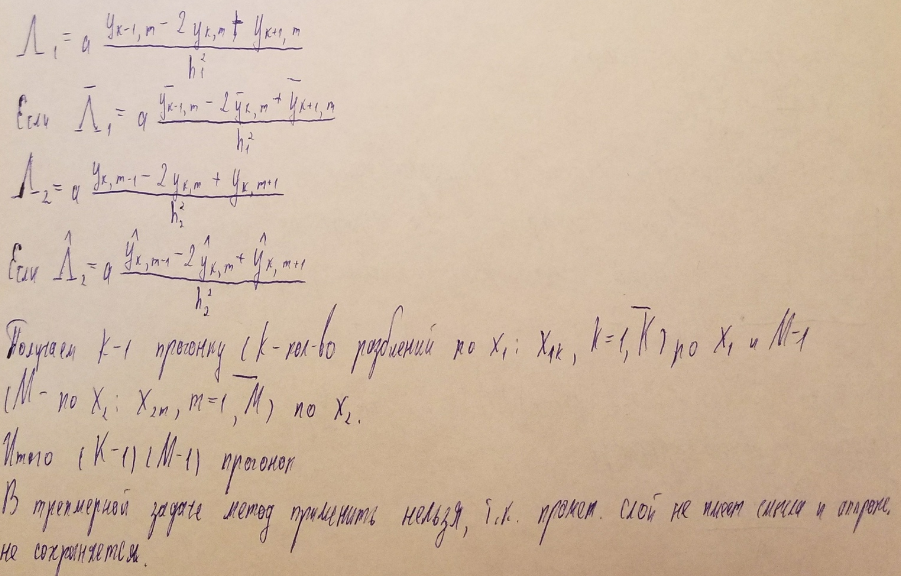
\includegraphics[width=7.0in]{../pics/39_4.png}\\
	\section{Локально-одномерный метод для решения многомерных уравнений в частных производных.}
	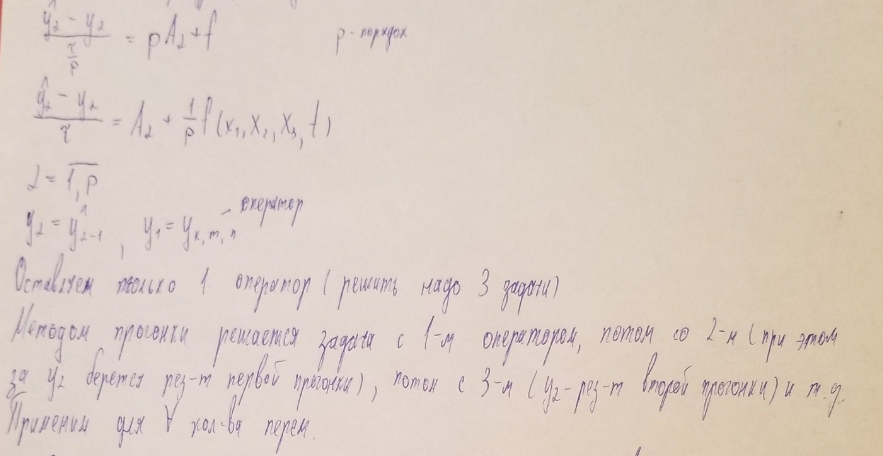
\includegraphics[width=7.0in]{../pics/40.png}\\\\		
	\section{Вероятностный метод для решения многомерных уравнений в частных производных.}
	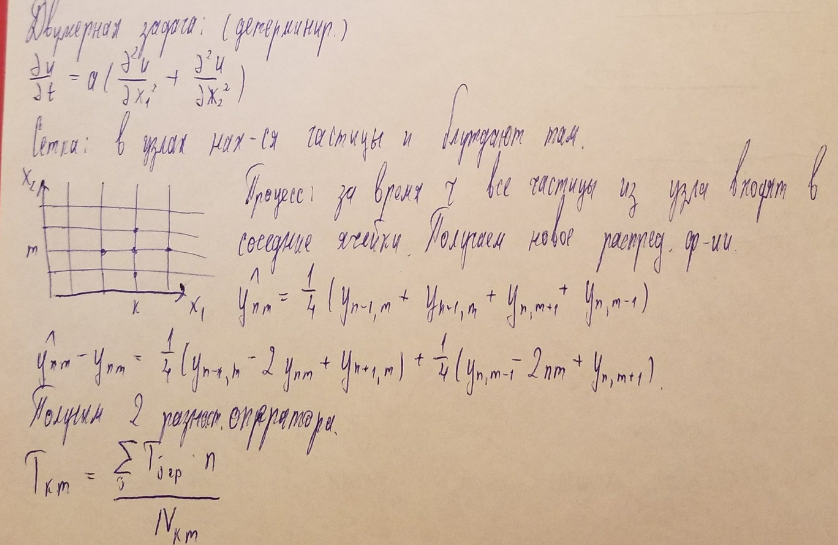
\includegraphics[width=7.0in]{../pics/41.png}\\\\
	
\end{document}